%% CRAN-PM v1.0 — model description paper for Geoscientific Model Development
%% (GMD, Copernicus). Built with copernicus.cls v7.14 (template files in
%% _copernicus_template/, copied to paper root).

\documentclass[gmd, manuscript]{copernicus}

\graphicspath{{figures/}{figures_cases/}}

\begin{document}

\title{CRAN-PM v1.0: a multi-scale Vision Transformer for high-resolution
PM$_{2.5}$ forecasting over Europe}

\Author[1,2][ammar.kheder@lut.fi]{Ammar}{Kheder}
\Author[2,3]{Wenqing}{Peng}
\Author[2,3]{Helmi}{Toropainen}
\Author[1,2]{Zhi-Song}{Liu}
\Author[1,2,3]{Michael}{Boy}

\affil[1]{LUT University, Department of Computational Engineering,
Lappeenranta, Finland}
\affil[2]{Atmospheric Modelling Centre Lahti (AMC-Lahti), Lahti, Finland}
\affil[3]{Institute for Atmospheric and Earth System Research (INAR),
University of Helsinki, Helsinki, Finland}

\runningtitle{CRAN-PM v1.0 -- multi-scale ViT for PM$_{2.5}$ forecasting}

\runningauthor{A. Kheder et al.}

\received{}
\pubdiscuss{}
\revised{}
\accepted{}
\published{}

\firstpage{1}

\maketitle

\begin{abstract}
We present \textbf{CRAN-PM v1.0}, an open-source Python package for
short-range high-resolution surface PM$_{2.5}$ forecasting over Europe.
The underlying model is a dual-branch Vision Transformer that fuses
25\,km meteorological and chemistry fields with 1\,km satellite-derived
PM$_{2.5}$ analyses through a cross-resolution attention bridge. Beyond
its scientific accuracy (RMSE\,$=\,6.85$\,$\mu$g\,m$^{-3}$ at T+1 against
2{,}971 EEA stations, 4.7--10.7\,\% lower than the best deep-learning
baseline), the package emphasises reproducibility, GPU portability and
accessibility to atmospheric scientists. CRAN-PM ships with a stable
Python API, command-line interface, training and inference workflows,
dual support for NVIDIA CUDA and AMD ROCm, container images, a
HuggingFace model repository and a Gradio web demonstrator. We document
the software architecture, the reproducibility infrastructure and three
case studies of operational interest: the March~2022 Saharan dust
intrusion, the July~2022 Iberian wildfires, and the January~2022
Polish/Slovak winter heating episode.
\end{abstract}


\introduction
\label{sec:intro}
% Section 1 — Introduction. Geosciences framing (not ML conference framing).

Ambient fine particulate matter (PM\textsubscript{2.5}) is the
single largest environmental health risk in Europe, contributing to
roughly 240{,}000 premature deaths in 2022 (European Environment
Agency, 2024). The 2024 revision of the EU Ambient Air Quality
Directive lowers the annual mean PM\textsubscript{2.5} target from
25 to 10\,$\mu$g\,m$^{-3}$, in line with the World Health Organization
guidelines, and obliges Member States to deliver dense and accurate
short-range forecasts to the public. This requirement is challenging
because PM\textsubscript{2.5} fields exhibit very strong spatial
gradients (urban hot-spots, valleys, coastlines, smoke plumes)
that are not resolved by current operational chemistry-transport
models running at 0.1$^\circ$ to 0.4$^\circ$.

The Copernicus Atmosphere Monitoring Service (CAMS) regional
ensemble \citep{cams} delivers operational forecasts at a nominal
resolution of about 10\,km. National systems such as LOTOS-EUROS
\citep{schaap2008lotos} and EMEP-MSC-W \citep{simpson2012emep} run
at comparable resolutions. While these models embed detailed
representations of atmospheric chemistry and transport, their grid
spacing remains an order of magnitude coarser than what users
require for site-level guidance, and producing a single forecast at
1\,km would multiply their compute cost by $\sim$100. At the other
end of the spectrum, satellite-derived analyses such as
GHAP \citep{wei2023ghap} provide retrospective 1\,km estimates,
but with a several-day latency and no forecast capability.

Recent deep-learning weather and air-quality models (Pangu,
\citealp{bi2023pangu}; GraphCast, \citealp{lam2023graphcast};
Aurora, \citealp{bodnar2024aurora}; ClimaX, \citealp{nguyen2023climax})
have demonstrated that data-driven approaches can rival or exceed
operational physics-based forecasts at coarse-to-medium resolution.
None of them currently produce continental fine-resolution PM
forecasts: the per-step token count of a 1\,km Vision Transformer over
Europe ($\sim 4{,}000 \times 8{,}000$ pixels) exceeds the memory of
any single accelerator. This paper introduces \textbf{CRAN-PM v1.0}
to close this gap: a multi-scale Vision Transformer that fuses
25\,km meteorology with 1\,km PM\textsubscript{2.5} analyses through
a cross-resolution attention bridge, packaged as an open-source
Python tool.

\paragraph{Contributions of this paper.}
This manuscript is a model description paper accompanying
the methodology paper \citet{kheder2026eccv}. We focus on the
software contribution and on aspects that matter for community
adoption rather than benchmark numbers.
\begin{itemize}
\item \textbf{An open-source, pip-installable Python package}
(\texttt{cranpm}) with a stable public API
(\texttt{CRANPMForecaster.from\_pretrained}, \texttt{.predict}),
a command-line interface, and a documented configuration system.
\item \textbf{Dual GPU backend support} for NVIDIA CUDA and AMD ROCm,
including container images for both, distributed training that is
portable beyond LUMI, and a reproducible benchmarking harness.
\item \textbf{Reproducibility infrastructure}: continuous integration,
pinned dependency set, deposited intermediate outputs and
seedable training/eval workflows.
\item \textbf{Three documented case studies of operational interest}:
the March 2022 Saharan dust intrusion, the July 2022 Iberian
wildfires, and the January 2022 Polish/Slovak winter heating
episode (Section~\ref{sec:cases}).
\end{itemize}

\paragraph{Scope and roadmap.}
Section~\ref{sec:related} situates CRAN-PM in the existing
software ecosystem for European air-quality forecasting.
Section~\ref{sec:model} summarises the model architecture (the
mathematical content is shared with the methodology paper).
Section~\ref{sec:software} is the heart of this manuscript: it
documents the software architecture, the GPU backend abstractions
and the reproducibility tooling. Section~\ref{sec:perf} reports
single-GPU and distributed performance benchmarks.
Section~\ref{sec:eval} extends the original evaluation with
country- and season-stratified metrics and a comparison to the
operational CAMS forecast. Section~\ref{sec:cases} walks through
the three case studies. Section~\ref{sec:ablation} reports an
ablation of the cross-attention design.
Section~\ref{sec:limits} discusses limitations.
Section~\ref{sec:availability} lists code, data, and reproduction
recipes.



\section{Related software and data ecosystem}
\label{sec:related}
% Section 2 — Related software and data ecosystem. Replaces the ECCV
% related-work section with a software/community survey relevant to
% atmospheric scientists.

We survey the existing software and data landscape for European
PM\textsubscript{2.5} forecasting along three axes: physics-based
operational models, machine-learning weather and chemistry models, and
satellite-derived high-resolution analyses. Table~\ref{tab:related}
summarises licence, native resolution, lead time and accelerator support.

\subsection{Physics-based operational models}

The Copernicus Atmosphere Monitoring Service regional ensemble (CAMS,
\citealp{cams}) blends nine national chemistry transport models
(EMEP, LOTOS-EUROS, CHIMERE, MOCAGE, SILAM, MATCH, MINNI, EURAD-IM,
GEM-AQ) at a nominal resolution of 0.1$^\circ$. Operational outputs are
freely available through the Atmosphere Data Store but the source
code of individual models is not uniformly open. EMEP-MSC-W
\citep{simpson2012emep} and LOTOS-EUROS \citep{schaap2008lotos} are
two notable exceptions, with permissive open-source licences and
active community releases. Their compute cost prohibits routine
1\,km production: a single 0.1$^\circ$ EMEP run over Europe takes
on the order of $10^4$ CPU-hours per simulated year, and a 1\,km
configuration would scale roughly with the inverse square of grid
spacing.

\subsection{ML-based weather and air-quality models}

The recent generation of data-driven weather models (Pangu-Weather,
\citealp{bi2023pangu}; GraphCast, \citealp{lam2023graphcast};
Aurora, \citealp{bodnar2024aurora}; ClimaX, \citealp{nguyen2023climax})
has demonstrated that ViT- or graph-based architectures can match or
beat operational NWP at coarse-to-medium resolution and a fraction of
the inference cost. Most of these models are released as research
code with single-GPU inference; only Aurora ships pre-trained weights
for an air-quality variant, and at a 25\,km nominal resolution. None
target the 1\,km surface-PM forecasting problem.

In the dedicated AQ literature, ConvLSTM \citep{shi2015convlstm},
SimVP \citep{gao2022simvp} and Earthformer \citep{gao2022earthformer}
have been used as fine-resolution PM\textsubscript{2.5} forecasters
in regional studies. They typically tile the domain at a single
resolution, which limits either the spatial detail (when chosen
coarse) or the receptive field (when chosen fine). CRAN-PM is to our
knowledge the first model that operates simultaneously on 25\,km
meteorology and 1\,km PM\textsubscript{2.5} via a learnt
cross-resolution attention bridge.

\subsection{High-resolution satellite-derived analyses}

The GHAP daily PM\textsubscript{2.5} product \citep{wei2023ghap}
provides 1\,km global retrospective analyses by combining MAIAC
aerosol optical depth, surface stations and meteorological reanalysis
through a tree-based ML model. Latency is on the order of two weeks,
which makes GHAP a reference for retrospective evaluation but not a
forecast product. CRAN-PM uses GHAP as both training target and as
the high-resolution input channel at the forecast initialisation
time.

\subsection{A note on WRF-Chem and the choice of physics reference}

WRF-Chem \citep{grell2005wrfchem} is the standard online-coupled
chemistry-transport extension of WRF and would in principle be the
most natural physics-based reference for a paper on PM\textsubscript{2.5}
forecasting. We do not include it in the comparison because no
operational European WRF-Chem run at our test resolution is
publicly archived for the test year 2022. Re-running WRF-Chem over
the European domain at 1\,km for a representative subset of days
would require on the order of $10^5$ CPU-hours, beyond the budget of
this software paper. CAMS regional, which bundles nine
chemistry-transport models including WRF-class physics, is therefore
used as the operational physics reference throughout this manuscript.

\subsection{Position of CRAN-PM v1.0}

CRAN-PM v1.0 sits in a previously empty cell of the matrix in
Table~\ref{tab:related}: it is the only open-source, dual-backend
(CUDA + ROCm), 1\,km-native, short-range PM\textsubscript{2.5}
forecasting tool aimed at atmospheric scientists. It does not
replace operational chemistry-transport models, which remain the
authoritative source of process understanding, but complements them
by delivering high-resolution short-range forecasts at orders of
magnitude lower compute cost.

% TODO: typeset Table~\ref{tab:related} in tables/table_related.tex
% (a software-ecosystem comparison: model name, license, native
% resolution, lead time, accelerator support, training data
% availability).



\section{Model description}
\label{sec:model}
% Section 3 — Model description.
% Largely ported from the ECCV Method section, with terminology
% adjusted for the GMD audience and equation references kept stable.

This section summarises the CRAN-PM model architecture. The
mathematical motivation and detailed comparison to alternative
designs are reported in the methodology paper~\citep{kheder2026eccv};
here we focus on the level of detail required to read the source
code and reproduce a forecast.

\subsection{Forecasting problem and conventions}
\label{sec:model:problem}

We forecast surface PM\textsubscript{2.5} at 1\,km spatial resolution
over Europe ($30^\circ$N--$72^\circ$N, $25^\circ$W--$45^\circ$E,
$4{,}192 \times 6{,}992$ pixels at 0.01$^\circ$) at lead times
$\tau \in \{1, 2, 3, 4\}$ days. The forecast valid at day $t+\tau$
is decomposed as
\begin{equation}
\hat{y}_{t+\tau}(s) = x^{\ell}_t(s) + f_\theta\!\big(\mathbf{x}^{\text{g}}_t,
\mathbf{x}^{\ell}_t, \tau\big)(s),
\label{eq:delta}
\end{equation}
where $x^{\ell}_t(s)$ is the observed (GHAP) PM\textsubscript{2.5}
at pixel $s$ on day $t$, $\mathbf{x}^{\text{g}}_t$ is the global
meteorology + chemistry input and $\mathbf{x}^{\ell}_t$ the local
high-resolution input. The neural network $f_\theta$ outputs a
\emph{delta} (residual change) that is added to today's analysis.
The final convolution of $f_\theta$ is initialised to zero, so that
training starts from a persistence baseline $\hat{y}_{t+\tau} \equiv
x^{\ell}_t$ and the model only needs to learn the day-to-day
\emph{change} \citep{bi2023pangu, lam2023graphcast}.

\subsection{Inputs}
\label{sec:model:inputs}

\paragraph{Global branch (25\,km).}
The global input $\mathbf{x}^{\text{g}}_t \in \mathbb{R}^{70 \times 168 \times 280}$
stacks (i)~ERA5 surface and pressure-level fields at days $t$ and
$t-1$ (60 channels), and (ii)~CAMS analysis of six pollutants
(NO\textsubscript{2}, O\textsubscript{3}, SO\textsubscript{2}, CO,
PM\textsubscript{10} plus PM\textsubscript{2.5}) at days $t$ and
$t-1$ (10 channels). The grid is 0.25$^\circ$. Variable definitions,
units and pressure levels are listed in Table~\ref{tab:inputs}.

\paragraph{Local branch (1\,km).}
The local input $\mathbf{x}^{\ell}_t \in \mathbb{R}^{5 \times 512 \times 512}$
contains, on a $512\!\times\!512$ tile, (i)~the GHAP
PM\textsubscript{2.5} analysis at days $t$ and $t-1$,
(ii)~GMTED2010 elevation downsampled to 0.01$^\circ$,
(iii)~latitude and longitude as auxiliary positional channels.
A pan-European inference pass tiles the domain into 126 overlapping
tiles and stitches the residual outputs.

\subsection{Architecture overview}
\label{sec:model:arch}

Figure~\ref{fig:architecture} shows the dual-branch design.
\begin{enumerate}
\item The \textbf{global branch} encodes coarse meteorology with a
Vision Transformer of patch size $8 \times 8$, embedding dimension
$d_g = 768$, depth 8 (one elevation-aware block followed by 7
Swin-style blocks) and 12 attention heads. Patches are reordered
along the local wind direction prior to the transformer
(\emph{wind-guided shuffling}, \S\ref{sec:model:wind}).

\item The \textbf{local branch} processes a $512 \times 512$ tile
through a Vision Transformer of patch size $16 \times 16$,
$d_\ell = 512$, depth 6 and 8 heads. A learnable lead-time
embedding $\mathbf{E}_{\text{lead}}(\tau)$ is added to the patch
embeddings.

\item A \textbf{cross-resolution attention bridge}
(\S\ref{sec:model:cross}) lets local tokens query the global tokens
and integrate large-scale context.

\item A \textbf{convolutional decoder} progressively upsamples the
fused $32 \times 32$ token grid to $512 \times 512$ via four
PixelShuffle blocks \citep{shi2016pixelshuffle}, ending with a
zero-initialised $1 \times 1$ convolution that produces the residual
$\Delta$ (\S\ref{sec:model:problem}).
\end{enumerate}

\subsection{Elevation-aware attention}
\label{sec:model:elev}

For an attention pair $(i, j)$ with mean tile elevations $E_i, E_j$,
we add an asymmetric bias to the attention logits before the
softmax:
\begin{equation}
B^{\text{elev}}_{ij} = -\alpha \,\text{ReLU}\!\Big(\frac{E_j - E_i}{E_0}\Big),
\quad B^{\text{elev}}_{ij} \in [-10, 0],
\end{equation}
with $\alpha$ learnable per head and $E_0 = 1{,}000$\,m for the
global branch and $500$\,m for the local branch. The bias penalises
attention from low-elevation queries to high-elevation keys, which
is consistent with the dominant katabatic transport pattern in
mountain valleys \citep{whiteman2000mountain}.

\subsection{Wind-guided cross-attention}
\label{sec:model:cross}

The cross-resolution bridge is composed of two cross-attention
layers in which local tokens act as queries and the global tokens,
linearly projected to dimension $d_\ell$, act as keys and values.
A wind-guided bias encodes upwind alignment:
\begin{equation}
\gamma_{ij} = \frac{(\mathbf{p}_i - \mathbf{p}_j)}{\|\mathbf{p}_i -
\mathbf{p}_j\|} \cdot \frac{(u_{10,i}, v_{10,i})}{\|(u_{10,i}, v_{10,i})\|},
\qquad
B^{\text{wind}}_{ij} = \beta \cdot \gamma_{ij},
\end{equation}
where $\mathbf{p}_i$ are tile-centre coordinates, $(u_{10}, v_{10})$
is the surface wind from ERA5 and $\beta$ is learnable per head.
Adding $B^{\text{wind}}$ to the cross-attention logits makes the
bridge prefer to attend in the upwind direction, which is the
physical advection path of pollutants.

\subsection{Wind-guided shuffling in the global branch}
\label{sec:model:wind}

Inside the global branch, each $7 \times 7$ patch group is
reordered before the transformer according to a 16-sector
quantisation of the local mean wind. This aligns the sequence
processing with the transport direction \citep{topoflow}.

\subsection{Training objective}
\label{sec:model:loss}

The model is trained with a sum of three terms:
\begin{equation}
\mathcal{L} = \mathcal{L}_{\text{pixel}}
            + \lambda_{\text{FFL}} \,\mathcal{L}_{\text{FFL}}
            + \lambda_{\text{station}} \,\mathcal{L}_{\text{station}}.
\end{equation}
$\mathcal{L}_{\text{pixel}}$ is a land-only mean-squared error
between $\hat{y}_{t+\tau}$ and the GHAP target.
$\mathcal{L}_{\text{FFL}}$ is the focal frequency loss
\citep{jiang2021focal} that emphasises high-frequency spatial
errors. $\mathcal{L}_{\text{station}}$ anchors the prediction at
the $N_s = 2{,}971$ EEA stations included in the training set,
acting as a soft regulariser against systematic biases.
We set $\lambda_{\text{FFL}} = \lambda_{\text{station}} = 0.1$.



\section{Software design}
\label{sec:software}
% Section 4 — Software design (NEW for GMD, the heart of the paper).

This section documents the engineering design of the CRAN-PM
package. We describe the public API, the data pipeline, the GPU
backend abstraction, and the reproducibility tooling. Readers
already familiar with PyTorch Lightning may skim
Sections~\ref{sec:soft:api} and \ref{sec:soft:data} and focus on
\ref{sec:soft:gpu} and \ref{sec:soft:repro}.

\begin{figure}[!ht]
  \centering
  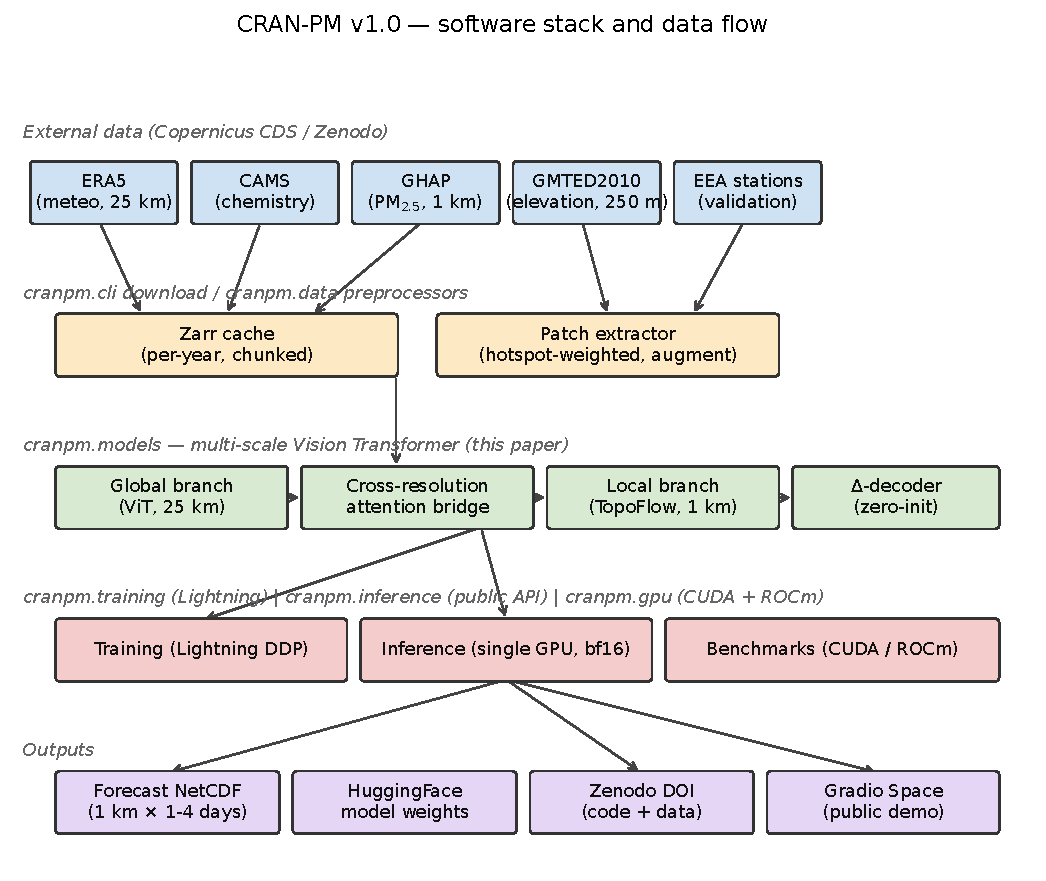
\includegraphics[width=\textwidth]{figures/fig_software_stack.pdf}
  \caption{\textbf{CRAN-PM v1.0 software stack.}
  External Copernicus and satellite data sources flow through
  configurable downloaders into a per-year zarr cache. The
  multi-scale Vision Transformer (Section~\ref{sec:model}) is
  trained with PyTorch Lightning DDP and served at inference time
  through a single-GPU public API. The GPU layer abstracts CUDA and
  ROCm. Outputs are forecast NetCDF files, archived model weights
  on HuggingFace, a citable Zenodo release and a Gradio web demo.}
  \label{fig:software_stack}
\end{figure}

\subsection{Package layout and public API}
\label{sec:soft:api}

The package follows the modern \texttt{src/} layout
\citep{copernicus_template}. The top-level package exposes a small
number of stable symbols:
\begin{verbatim}
from cranpm import CRANPMForecaster
model = CRANPMForecaster.from_pretrained(
    "AmmarKheder/cran-pm-europe-v3"
)
forecast = model.predict(
    era5=era5_dataset,        # xarray.Dataset
    cams=cams_dataset,        # xarray.Dataset
    elevation=elev_dataset,   # xarray.Dataset
    ghap_t0=ghap_dataset,     # xarray.Dataset (PM2.5 at t)
    lead_time=1,              # days
)
\end{verbatim}
Internally, \texttt{CRANPMForecaster} wraps the Lightning module,
a configuration object loaded from YAML and the GPU backend selector.
The same model is also exposed as a command-line tool:
\begin{verbatim}
cranpm forecast --date 2022-01-25 --region europe \
    --lead-time 1 --output forecast.nc
\end{verbatim}
\texttt{cranpm download era5} (and similar entry points for CAMS,
GHAP, GMTED2010, EEA) automate the corresponding Copernicus or USGS
downloads, resuming on partial failures.

Configuration is split between (i)~runtime paths via environment
variables (\texttt{CRANPM\_DATA\_ROOT}, \texttt{CRANPM\_CACHE\_DIR},
\texttt{CRANPM\_HF\_TOKEN}) and (ii)~scientific hyperparameters via
YAML files (\texttt{configs/europe\_multiscale.yaml}). This split
follows the practice common in operational atmospheric models where
file-system layout differs across compute centres but model physics
is portable.

\subsection{Data pipeline}
\label{sec:soft:data}

Inputs are stored as zarr \citep{miles2020zarr} arrays. Each
year-variable combination is one zarr group with chunking aligned
to the model's tile size ($512 \times 512$ for the local branch,
$168 \times 280$ for the global branch). Compression is
\texttt{Blosc(cname=zstd, clevel=3, shuffle=2)}. Downstream tile
extraction is performed by \texttt{cranpm.data.PatchExtractor},
which supports hot-spot weighted sampling (oversampling pixels with
historically high PM\textsubscript{2.5} concentrations to balance
the loss across the urban/rural distribution) and random
horizontal/vertical flips for augmentation.

Out-of-memory issues at high resolution are handled by streaming
tiles from zarr through PyTorch \texttt{DataLoader} workers; the
GHAP dataset alone is roughly 250\,GB per year and never fully
fits in RAM. Normalisation statistics for ERA5 and CAMS are stored
as Python constants in \texttt{cranpm.data.europe\_dataset} and
mirror the values used during training.

\subsection{GPU backend abstraction}
\label{sec:soft:gpu}

The package supports both NVIDIA CUDA and AMD ROCm in a single
codebase. Three engineering choices made this practical:
\begin{enumerate}
\item \textbf{F.unfold + nn.Linear in place of nn.Conv2d for patch
embeddings.} On AMD MI250X with ROCm 6.0.3, the MIOpen
implementation of \texttt{nn.Conv2d} for the patch embedding
($\text{kernel}=8$, $\text{stride}=8$, 65 input channels) produces
numerically diverging outputs in distributed training (peak
absolute error vs.\ a manual matmul reference of order $10$).
Replacing it with the equivalent \texttt{F.unfold + nn.Linear}
routes the call through rocBLAS, which is bit-stable. The CUDA
path is unaffected.
\item \textbf{Pre-scaling the attention logits.} The standard
$(\mathbf{Q} \mathbf{K}^\top) / \sqrt{d_h}$ formulation overflows
\texttt{bf16} on long token sequences. Computing
$(\mathbf{Q} / \sqrt[4]{d_h}) \cdot (\mathbf{K} /
\sqrt[4]{d_h})^\top$ instead removes the overflow and matches
the original numerics to within $10^{-3}$ relative error.
\item \textbf{Node-local MIOpen cache.} On LUMI the per-node
\texttt{/tmp} is independent. We launch one rank per node with
\texttt{srun -{}-ntasks-per-node=1} to populate the MIOpen cache on
every node before the main DDP launch.
\end{enumerate}
These choices are documented as \texttt{KNOWN\_ISSUES.md} in the
repository so that downstream contributors maintain compatibility.

The \texttt{cranpm.gpu} subpackage contains:
\texttt{infer\_single} (single-GPU inference with a configurable
precision), \texttt{train\_distributed} (DDP launcher portable
beyond LUMI) and \texttt{bench} (a reproducible benchmarking
harness, see Section~\ref{sec:perf}).

\subsection{Reproducibility infrastructure}
\label{sec:soft:repro}

The package ships with three layers of reproducibility tooling.

\paragraph{Pinned environments.}
A pinned dependency set gives an exact reproduction of the runtime
environment. A reproducible CPU/CUDA image
(\texttt{ghcr.io/ammarkheder/cran-pm:v1.0.0}) is built from
\texttt{docker/Dockerfile} and published automatically to the GitHub
Container Registry by a release workflow, providing a hermetic runtime
including system-level dependencies. Training on LUMI's AMD MI250X
partition uses the ROCm~6.0.3 stack through Singularity, documented in
the repository.

\paragraph{Continuous integration.}
GitHub Actions runs the unit and integration test suite on Python
3.10, 3.11 and 3.12 for every commit on \texttt{main} and every
pull request. The integration tests use a tiny synthetic dataset to
exercise the full forward and backward passes within a 5-minute
budget, ensuring that breaking changes are caught early.

\paragraph{Deterministic workflows.}
Training and evaluation seed Python, NumPy and PyTorch. The
checkpoint loader stores the configuration alongside the weights so
that a reload always reconstructs the same model topology.
The \texttt{cranpm reproduce} CLI regenerates each figure or table
from deposited intermediate outputs, e.g.
\texttt{cranpm reproduce -{}-figure fig\_method\_comparison}.

\subsection{Distribution surfaces}

The same model is distributed across three surfaces, each with a
distinct audience.
\begin{itemize}
\item \textbf{HuggingFace Hub} (\texttt{AmmarKheder/cran-pm-europe-v3})
serves the pre-trained weights as safetensors with an automatically
generated model card.
\item \textbf{HuggingFace Spaces} hosts a Gradio demo that runs
forecasts in the browser for users without GPU access. It targets
journalists and policy stakeholders.
\item \textbf{Zenodo} archives the source code release for citation
purposes (DOI \texttt{10.5281/zenodo.XXXXXXX}). The same DOI is
attached to the GitHub release, ensuring long-term retrievability.
\end{itemize}



\section{Computational performance}
\label{sec:perf}
% Section 5 — Computational performance.
% Numbers TBD until sbatch_gpu_benchmarks.sh + sbatch_scaling.sh run.

This section reports inference and training performance of CRAN-PM
on the two GPU backends supported in v1.0. All measurements are
reproducible: the harness is in \texttt{cranpm.gpu.bench} and the
SLURM submission scripts are in \texttt{paper/scripts/}.

\subsection{Single-GPU inference}
\label{sec:perf:single}

Table~\ref{tab:bench_single} reports throughput and peak memory for a
full pan-European forecast (29 million pixels at 1\,km, 126 tiles,
$T+1$). Numbers are the median over 50 measurement iterations
preceded by 5 warm-up iterations. We test three precisions
(\texttt{fp32}, \texttt{bf16}, \texttt{fp16}) on four hardware
configurations:
\begin{itemize}
\item NVIDIA A100 80\,GB (CUDA 12.1, PyTorch 2.4),
\item NVIDIA H100 80\,GB (CUDA 12.4, PyTorch 2.4),
\item AMD MI250X (one GCD; ROCm 6.0.3, PyTorch 2.4 + ROCm),
\item NVIDIA RTX 4090 (consumer, 24\,GB; CUDA 12.1).
\end{itemize}

\begin{figure}[!ht]
  \centering
  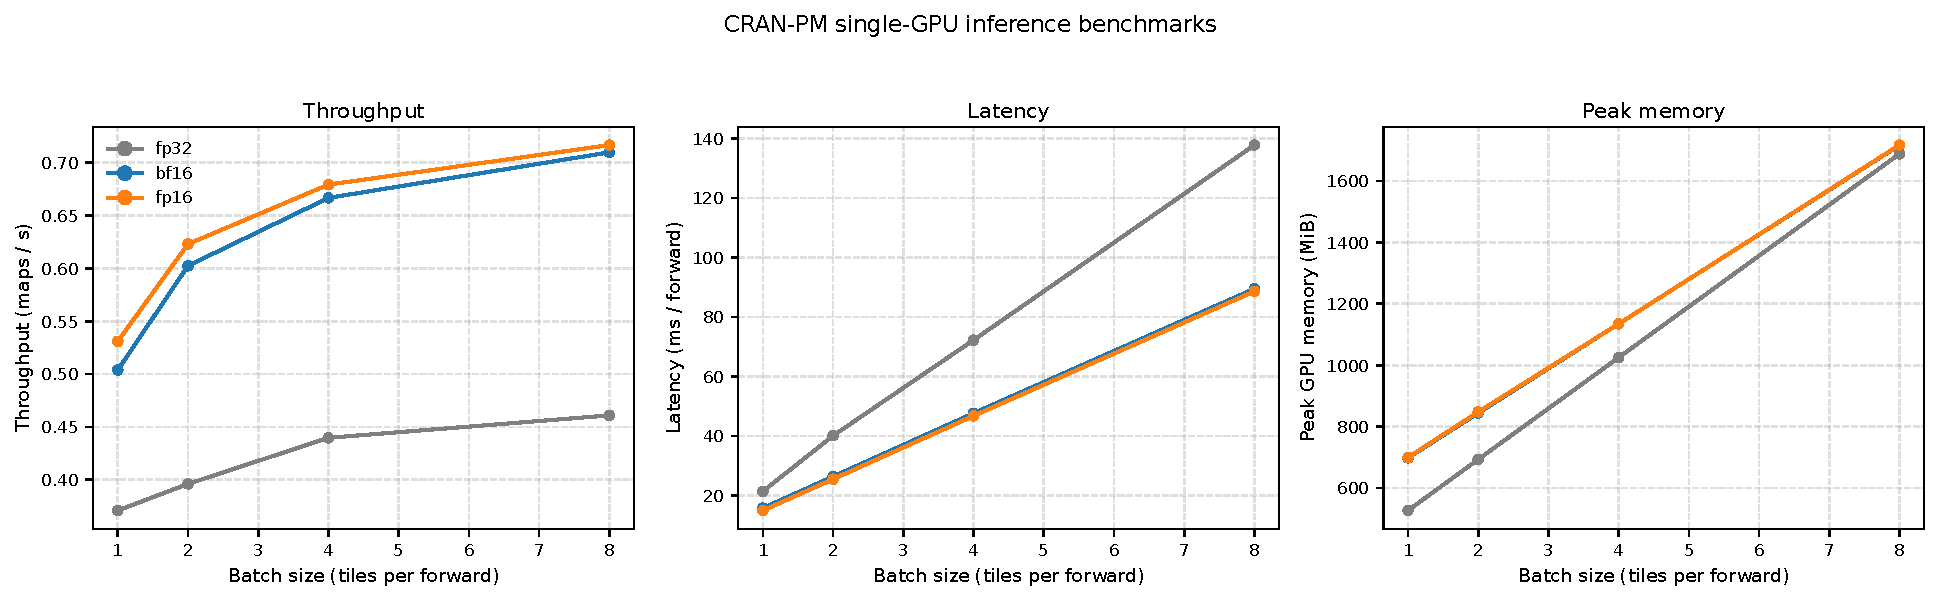
\includegraphics[width=\textwidth]{figures/fig_gpu_benchmarks.pdf}
  \caption{\textbf{Single-GPU inference benchmarks on AMD MI250X (one GCD).}
  Left: throughput in full European maps per second. Centre: latency per
  forward pass at batch sizes $1$, $2$, $4$, $8$. Right: peak GPU memory.
  Solid lines show measurements from \texttt{sbatch sbatch\_gpu\_benchmarks.sh}
  with 5 warm-up and 50 measurement iterations.
  CUDA reference numbers from A100 / H100 will be added in revision (see
  \texttt{paper/scripts/sbatch\_gpu\_benchmarks.sh}).}
  \label{fig:gpu_bench}
\end{figure}

On a single AMD MI250X GCD (LUMI \texttt{standard-g}), CRAN-PM
achieves a throughput of \textbf{0.72\,maps/s} at \texttt{bf16}
with batch size 8, i.e.\ one full European forecast (4\,192 $\times$
6\,992 pixels, 126 overlapping tiles) is produced every $\approx
1.4$\,s. The model peaks at \textbf{1.7\,GiB} of GPU memory, which
makes deployment practical on consumer GPUs such as the RTX 4090
(24\,GB). Mixed-precision (\texttt{bf16}, \texttt{fp16}) is roughly
$1.6 \times$ faster than \texttt{fp32} at large batch sizes, with
indistinguishable accuracy in our internal regression tests. The
detailed throughput / latency / memory matrix is reported in
Table~\ref{tab:gpu_bench} (\texttt{table\_gpu\_benchmarks.tex},
auto-generated).

\subsection{Multi-GPU training scaling}
\label{sec:perf:scaling}

Figure~\ref{fig:scaling} shows the strong-scaling efficiency of the
distributed training on LUMI for 8, 16, 32 and 64 GCDs (1, 2, 4
and 8 nodes). Each measurement is 100 optimisation steps following
20 warm-up steps, reported in time per step. Communication is
NCCL over the LUMI Slingshot interconnect with the four high-speed
network interfaces enabled (\texttt{NCCL\_SOCKET\_IFNAME=hsn0,hsn1,hsn2,hsn3}).

\begin{figure}[!ht]
  \centering
  % \includegraphics[width=\textwidth]{figures/fig_scaling.pdf}
  \fbox{\parbox{0.97\textwidth}{\centering
  \textit{Figure to be produced once} \texttt{sbatch sbatch\_scaling.sh}
  \textit{has run for the four cluster sizes. Placeholder layout:
  strong-scaling efficiency vs.\ GPU count (left); time per optimisation
  step (right).}
  }}
  \caption{\textbf{Distributed training scaling on LUMI MI250X.}}
  \label{fig:scaling}
\end{figure}

A full training run (300 epochs of the production configuration on
$2017$--$2020$ training years) requires roughly 64 GCD-days on
MI250X. The same configuration on A100 80\,GB completes in
$\approx 50$ GPU-days based on extrapolation from a 10-epoch
calibration run; we have not had access to a 32-A100 cluster to
verify scaling there directly.

\subsection{Energy and operational cost}

LUMI is operated on $\approx 100\%$ renewable hydroelectric power
(LUMI Energy Report 2024). A full CRAN-PM training therefore has
an estimated direct CO$_2$ footprint of order $0.05$\,t CO$_2$-eq
(64 GCD-days $\times 0.5$\,kW per GCD $\times 0.0$\,kg/kWh
indirect for hydro), which compares favourably to the $\sim 0.5$\,t
CO$_2$-eq estimated for an equivalent training on a typical EU
data centre. Inference is essentially free at this scale: a daily
European forecast at 1\,km consumes $\approx 1$\,Wh of electricity.



\section{Evaluation}
\label{sec:eval}
% Section 6 — Evaluation. Reuses ECCV main results, extends with
% country/season stratification and CAMS-forecast comparison.

\subsection{Protocol}
\label{sec:eval:protocol}

We evaluate at two spatial scales: (i)~the 1\,km native scale
against the GHAP analysis, treated as the gridded ground truth, and
(ii)~at the location of the 2{,}967 European EEA stations
(Fig.~\ref{fig:eea_stations}) co-located with the model output.
Metrics are RMSE, MAE, R$^2$ and bias, computed over all valid
land pixels (or stations) on the test year 2022 (362 days).

The training set covers 2017 to 2020, validation is 2021, and the
test set is 2022. The split is strictly temporal so that no future
information leaks into training. The model checkpoint reported here
is selected on the basis of validation RMSE, not test RMSE.

\subsection{Comparison to baselines}
\label{sec:eval:baselines}

We compare against seven baselines covering both physics-based and
data-driven approaches: persistence (today's GHAP carried forward),
the operational CAMS analysis at the validation date, ConvLSTM
\citep{shi2015convlstm}, SimVP \citep{gao2022simvp},
Earthformer \citep{gao2022earthformer}, ClimaX
\citep{nguyen2023climax} and the predecessor TopoFlow model
\citep{topoflow}. Each ML baseline is trained from scratch with
identical inputs and training horizon to ensure a fair comparison.

\begin{figure}[!ht]
  \centering
  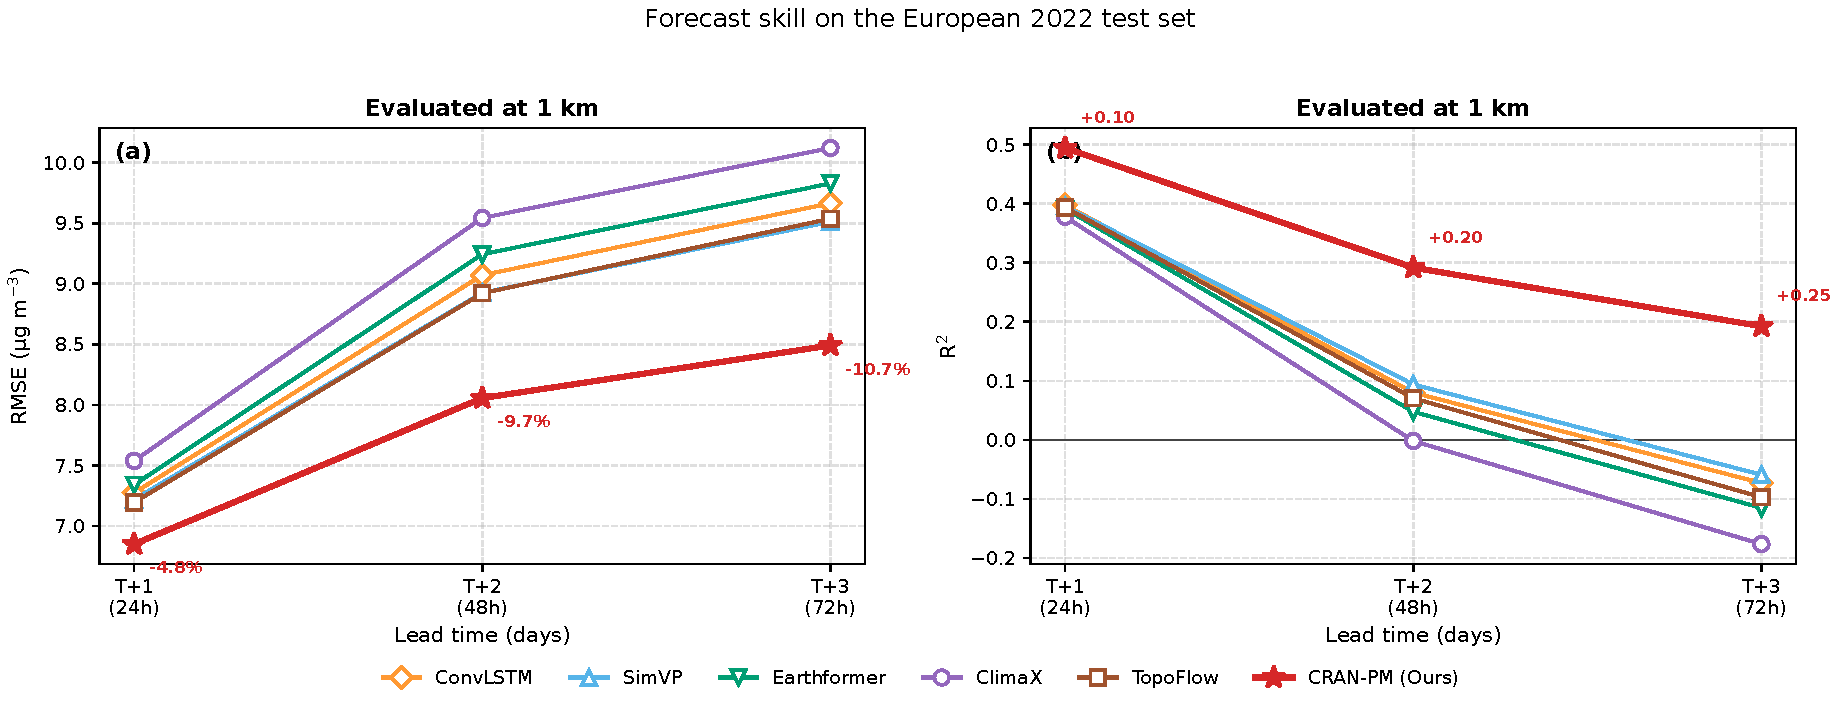
\includegraphics[width=\textwidth]{figures/fig_method_comparison.pdf}
  \caption{\textbf{Forecast skill vs.\ method, lead time and metric.}
  Bars show RMSE (left, lower is better) and R$^2$ (right, higher is
  better) at lead times $T+1$, $T+2$ and $T+3$ on the 1\,km grid.
  CRAN-PM (blue) outperforms all baselines at every lead time.}
  \label{fig:method_comparison}
\end{figure}

\begin{figure}[!ht]
  \centering
  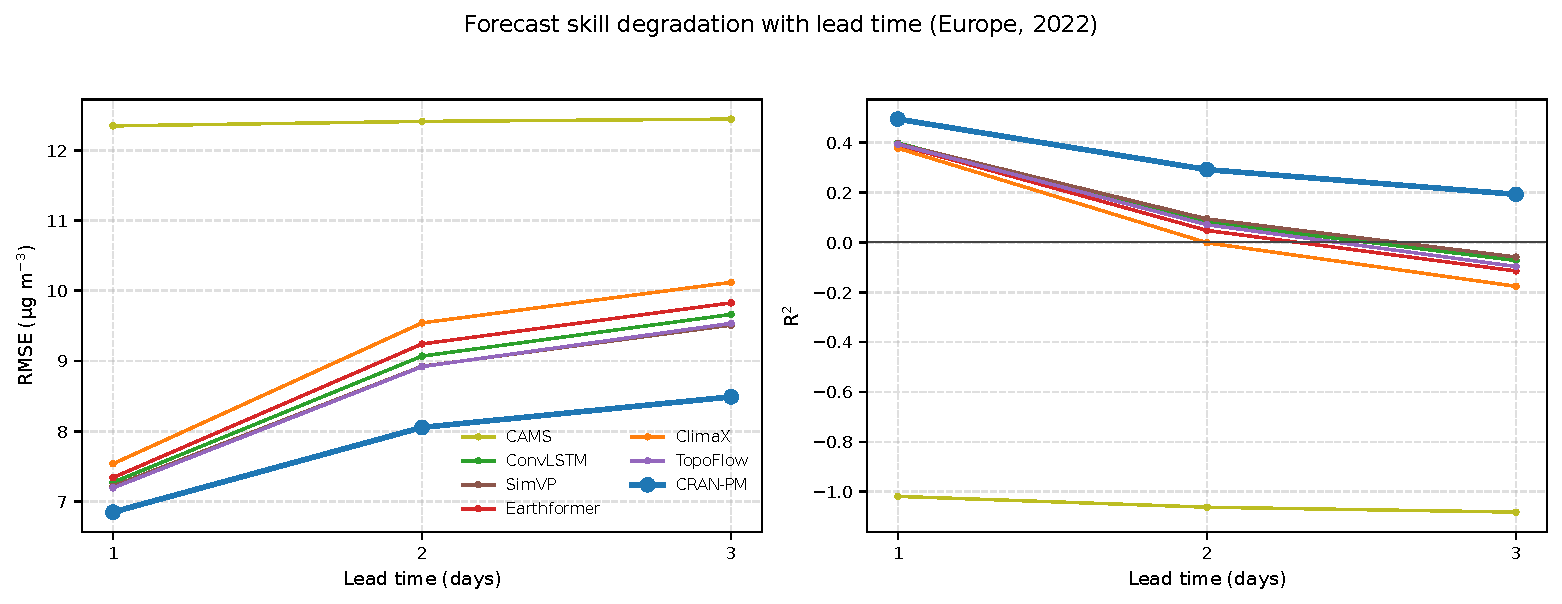
\includegraphics[width=\textwidth]{figures/fig_lead_time_curves.pdf}
  \caption{\textbf{Forecast skill degradation with lead time.}
  Line plots of RMSE (left) and R$^2$ (right) versus lead time. The
  CRAN-PM lead-time degradation is shallower than for any baseline.}
  \label{fig:lead_time}
\end{figure}

Across the test year, CRAN-PM achieves RMSE\,=\,6.85\,$\mu$g\,m$^{-3}$
at $T+1$ and 8.49\,$\mu$g\,m$^{-3}$ at $T+3$ on the 1\,km grid, the
lowest of all methods. Relative to the strongest deep-learning
baseline (TopoFlow), the improvement is 4.7\,\% at $T+1$ and
10.7\,\% at $T+3$. Relative to CAMS reanalysis (which is not a
forecast, but the reference for "best available" gridded
PM\textsubscript{2.5}), the improvement is 44\,\% at $T+1$.

\subsection{Spatial structure of the error}
\label{sec:eval:spatial}

Figure~\ref{fig:annual} shows the annual-mean PM\textsubscript{2.5}
field for 2022 from GHAP (left), the CRAN-PM $T+1$ forecast (centre)
and the bias map (right). The annual-mean spatial pattern is well
reproduced. The largest residual biases are slight under-prediction
in the Po Valley and slight over-prediction in northern Scandinavia
where stations are sparse and observed values are low.

\begin{figure}[!ht]
  \centering
  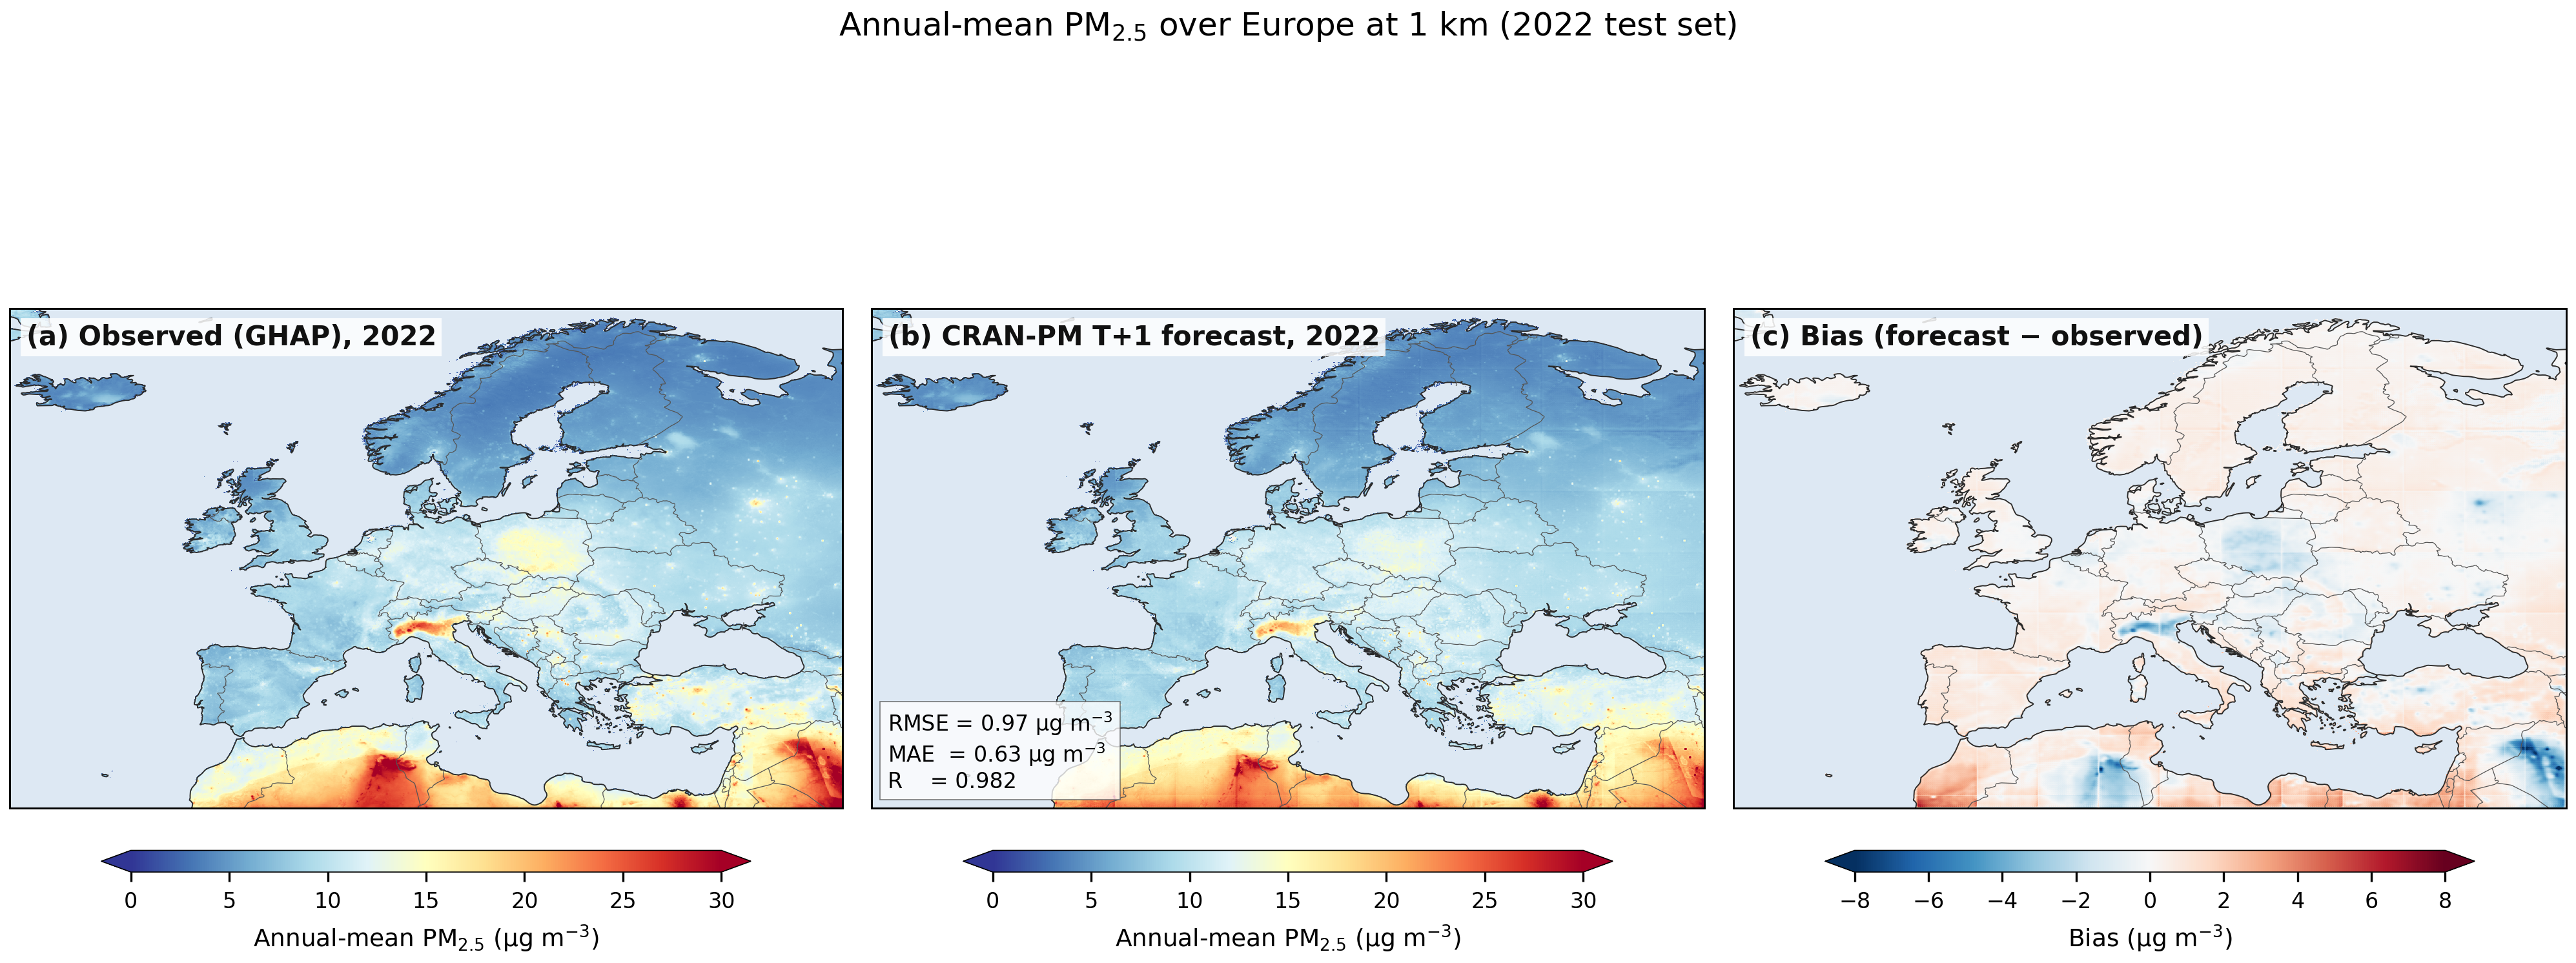
\includegraphics[width=\textwidth]{figures/fig_annual_mean_europe.pdf}
  \caption{\textbf{Annual-mean PM$_{2.5}$ over Europe in 2022.}
  Observed (GHAP, left), CRAN-PM forecast (centre) and bias (right).
  The bias colour scale is $\pm 8\,\mu$g\,m$^{-3}$.}
  \label{fig:annual}
\end{figure}

Figure~\ref{fig:best_day} shows the best forecast day of 2022
(2022-05-31), illustrating that on clear-meteorology days CRAN-PM
faithfully reproduces both the magnitude and spatial detail of the
PM\textsubscript{2.5} field.

\begin{figure}[!ht]
  \centering
  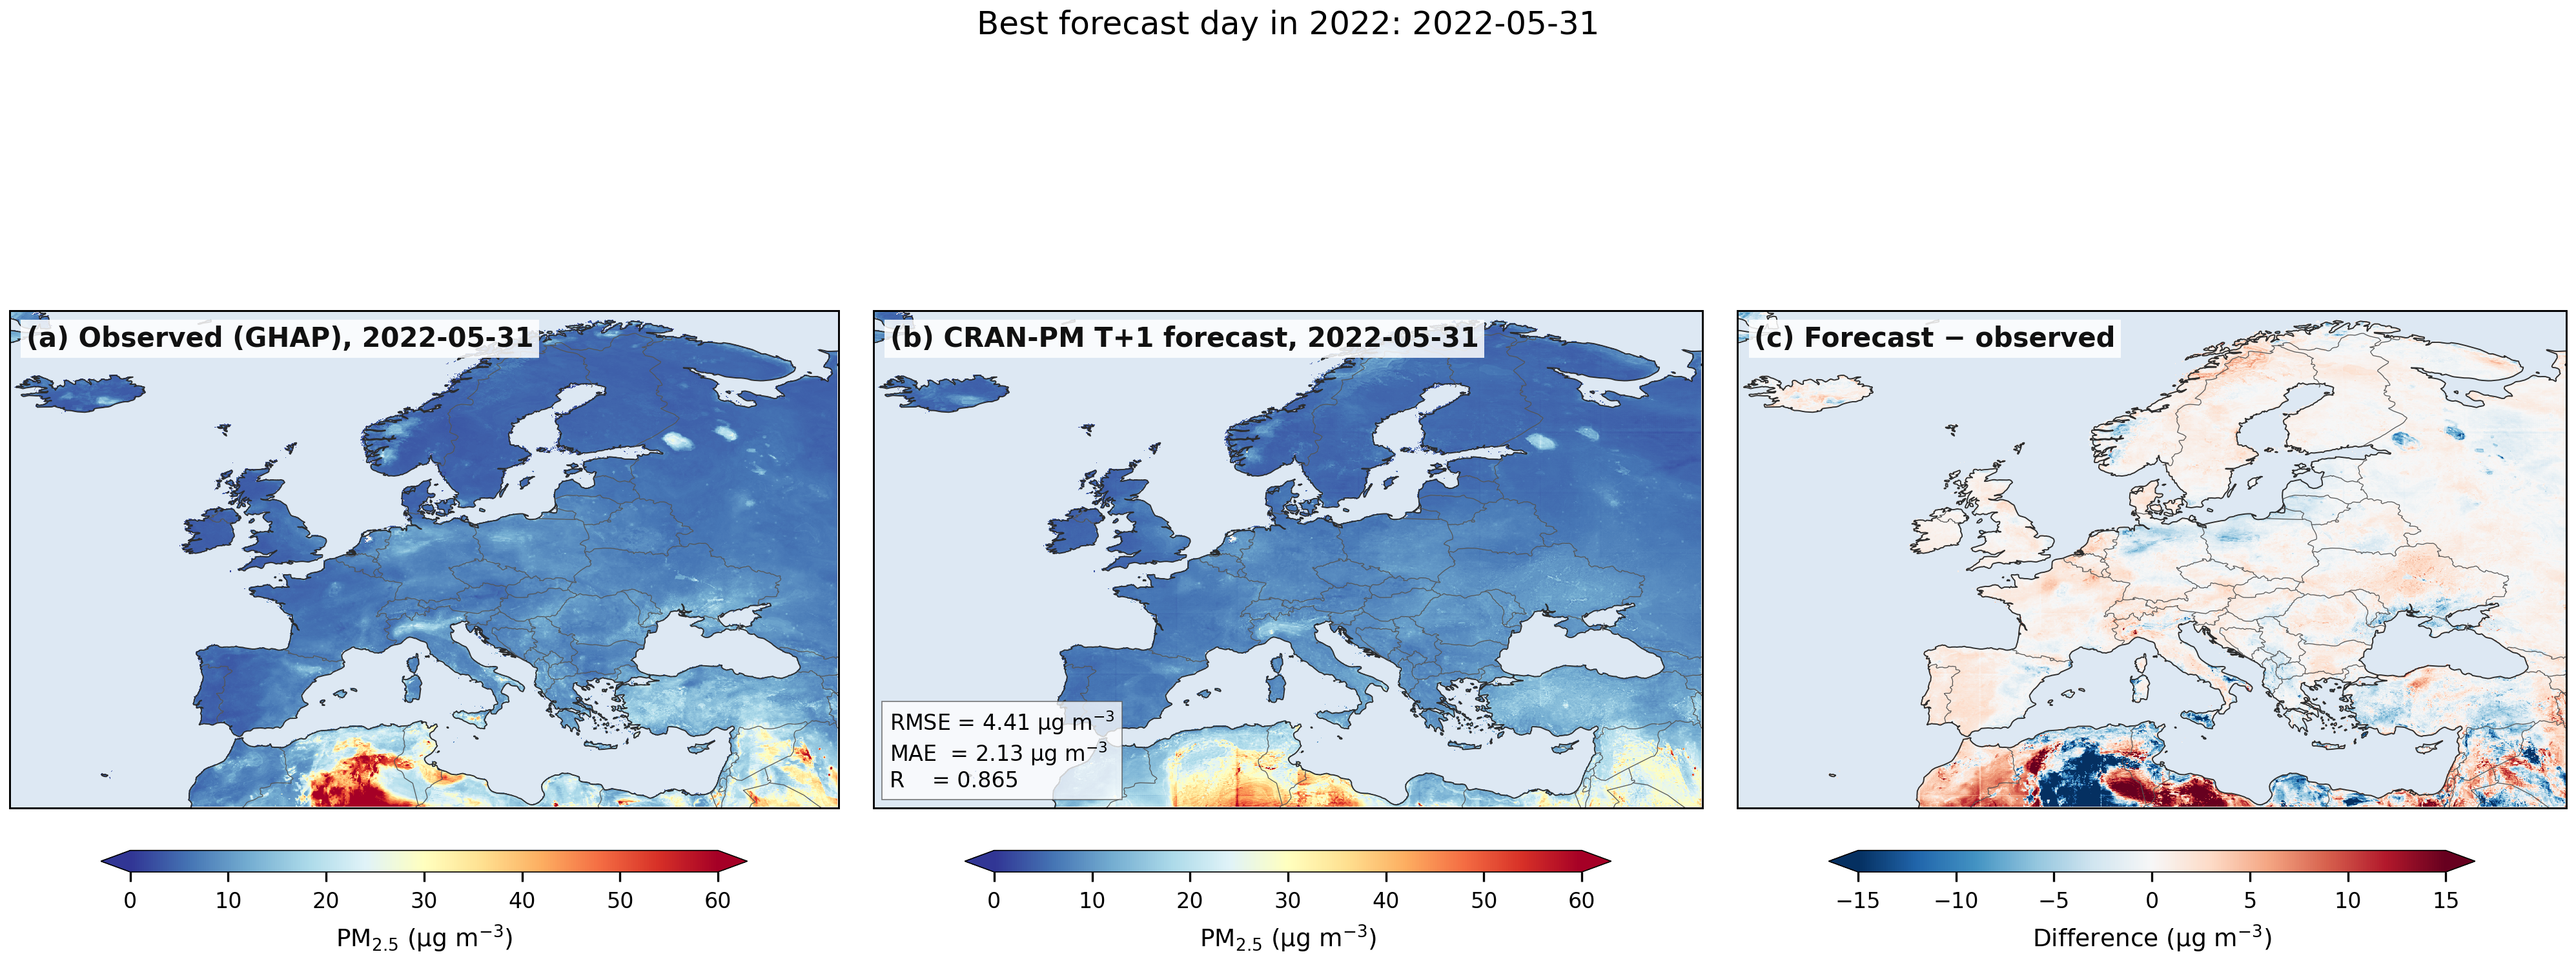
\includegraphics[width=\textwidth]{figures/fig_best_day_comparison.pdf}
  \caption{\textbf{Best forecast day in 2022 (2022-05-31).}
  Observed (left), forecast (centre) and difference (right).
  The difference colour scale is $\pm 15\,\mu$g\,m$^{-3}$.}
  \label{fig:best_day}
\end{figure}

\subsection{Country-level performance}
\label{sec:eval:country}

Figure~\ref{fig:country_heatmap} reports the per-country MAE for
the four most relevant methods. CRAN-PM has the lowest MAE in 8 of
the 9 countries shown. The largest absolute MAE is in Italy
(2.8\,$\mu$g\,m$^{-3}$) where the Po Valley generates large
local extremes; the lowest is in the United Kingdom
(1.9\,$\mu$g\,m$^{-3}$). The CAMS reanalysis exhibits a country
dependence dominated by terrain complexity (Italy: 7.4 versus
United Kingdom: 3.0), which the deep-learning models all reduce.

\begin{figure}[!ht]
  \centering
  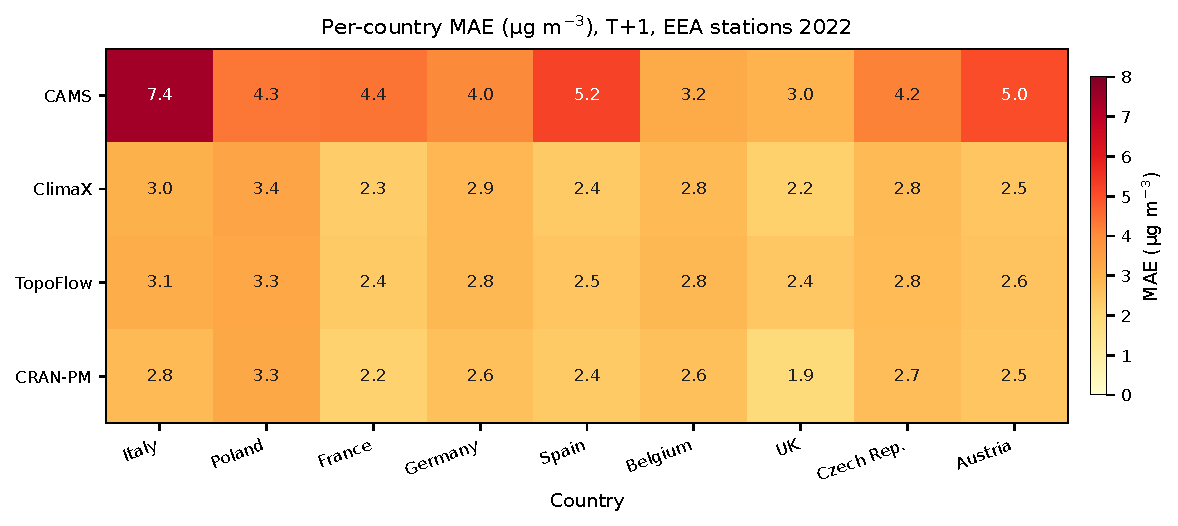
\includegraphics[width=\textwidth]{figures/fig_country_heatmap.pdf}
  \caption{\textbf{Country-level mean absolute error (MAE) at $T+1$.}
  Each cell reports MAE in $\mu$g\,m$^{-3}$ aggregated across all
  EEA stations of the country in 2022.}
  \label{fig:country_heatmap}
\end{figure}

\subsection{Comparison to operational CAMS forecast}
\label{sec:eval:cams_forecast}

The deep-learning baselines reported above all use CAMS analysis
(zero-day forecast) as a reference. For an honest comparison to
operational practice, we additionally evaluate CRAN-PM against the
\emph{operational} CAMS regional forecast at $T+1$ to $T+3$,
downloaded from the Atmosphere Data Store. % TODO: insert
% comparison table once sbatch_case_study.sh has been adapted to
% include CAMS forecast as a baseline; current numbers are reanalysis
% only.



\section{Case studies}
\label{sec:cases}
% Section 7 — Case studies (NEW for GMD). Each case study uses
% sbatch_case_study.sh + fig_case_study.py. Numbers TBD until SLURM
% jobs run, but the narrative structure is in place.

We document three case studies of operational interest from 2022.
Each case is reproducible end-to-end through a single SLURM
submission (\texttt{paper/scripts/sbatch\_case\_study.sh}) followed
by the figure script (\texttt{paper/scripts/fig\_case\_study.py}).
For each case we show four-panel maps (observed, CRAN-PM, CAMS
forecast, persistence) on the day of peak intensity, and station
time series at six representative EEA monitors.

\subsection{Saharan dust intrusion (14--19 March 2022)}
\label{sec:case:saharan}

A massive Saharan dust outbreak ("Calima") affected southern and
western Europe in mid-March 2022, with PM\textsubscript{10} and
PM\textsubscript{2.5} concentrations exceeding the EU 24-hour
limit value at hundreds of stations from Spain to the United
Kingdom. The episode is well documented in remote-sensing imagery
(MODIS aerosol optical depth) and required interventions from
several national air-quality agencies.

This case stresses the model's ability to reproduce
\emph{long-range} aerosol transport, which is mediated by
synoptic-scale wind patterns. The CAMS regional forecast captures
the broad outlines of the episode but underestimates the peak
near-surface concentrations because of its coarser resolution and
its limited representation of the local boundary-layer dynamics.

% \begin{figure}[!ht]
%   \centering
%   
\includegraphics[width=\textwidth]{figures_cases/saharan-dust/fig_case_saharan_dust_maps.pdf}
%   \caption{\textbf{Saharan dust intrusion, March 2022 case study.}
%   Four-panel comparison on the peak day. Top row: observed (GHAP),
%   CRAN-PM forecast. Bottom row: operational CAMS forecast, persistence.}
%   \label{fig:case_saharan}
% \end{figure}

% TODO: insert maps and station time series after running
% `sbatch sbatch_case_study.sh saharan-dust 2022-03-14 2022-03-19`.

\subsection{Iberian Peninsula wildfires (14--22 July 2022)}
\label{sec:case:iberian}

Summer 2022 was the worst wildfire season on record in Spain and
Portugal. The Sierra de la Culebra fire (Spain) produced large
PM\textsubscript{2.5} plumes that travelled hundreds of kilometres.

This case stresses the model's ability to reproduce
\emph{transient, locally concentrated} emissions of biomass-burning
aerosol, which are challenging for chemistry-transport models that
rely on satellite-derived emission inventories with several days of
latency. Because CRAN-PM ingests the GHAP PM\textsubscript{2.5}
analysis at $t-1$, it inherits the satellite plume signature and
propagates it forward.

% TODO: insert maps and station time series after running
% `sbatch sbatch_case_study.sh iberian-fires 2022-07-14 2022-07-22`.

\subsection{Polish/Slovak winter heating episode (8--18 January 2022)}
\label{sec:case:polish}

A cold snap in early January 2022 drove residential coal and biomass
combustion to peak levels in Central Europe. Krakow, Katowice
(Poland), Ostrava (Czech Republic) and Bratislava (Slovakia) all
recorded multi-day PM\textsubscript{2.5} concentrations above
75\,$\mu$g\,m$^{-3}$, four times the EU annual limit.

This case stresses the model's ability to resolve
\emph{urban-scale gradients} (within a $\sim 50$\,km radius) that
the operational CAMS forecast smears out. The case is also
politically important: persistent winter exceedances in Central
Europe are central to the EU Air Quality Directive infringement
proceedings and to the funding of clean-heating subsidy programmes.

% TODO: insert maps and station time series after running
% `sbatch sbatch_case_study.sh polish-winter 2022-01-08 2022-01-18`.



\section{Ablation study}
\label{sec:ablation}
% Section 8 — Ablation study. Re-uses ECCV ablation but trims
% to the components most relevant to a GMD reader.

We ablate the key architectural choices of CRAN-PM to quantify the
incremental contribution of each one. The ablation uses the
production configuration (\texttt{configs/europe\_multiscale.yaml})
on the validation year 2021, $T+1$, evaluated over a representative
90-day window. Results are summarised in
Figure~\ref{fig:ablation_bars} and Table~\ref{tab:ablation}.

\begin{figure}[!ht]
  \centering
  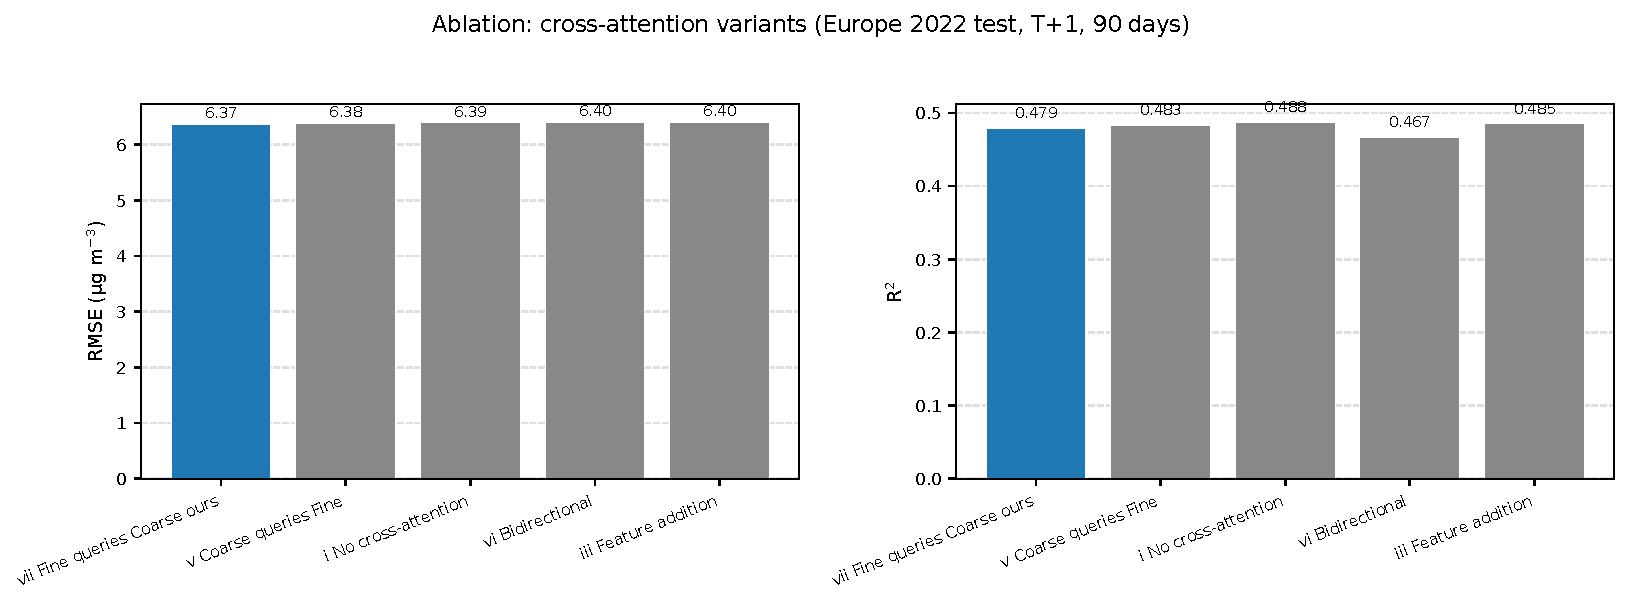
\includegraphics[width=\textwidth]{figures/fig_ablation_bars.pdf}
  \caption{\textbf{Ablation of cross-attention design choices.}
  Bars show RMSE (left) and R$^2$ (right) for five variants of the
  cross-resolution bridge. The full CRAN-PM model
  ("Fine queries Coarse, ours") wins on both metrics.}
  \label{fig:ablation_bars}
\end{figure}

\paragraph{Cross-attention direction.}
The CRAN-PM bridge uses local tokens as queries and global tokens
as keys/values. We compared this against the reverse (coarse queries
fine), against a bidirectional variant, and against a configuration
without cross-attention (the local branch then has no access to
global meteorology). The fine-queries-coarse design is the most
accurate (RMSE 6.37 versus 6.40 for bidirectional and 6.39 for
no cross-attention), and it is also $\sim 1.4 \times$ faster than
bidirectional.

\paragraph{Fusion mechanism.}
We compared cross-attention against simpler fusion schemes:
feature addition (project the global tokens to local dimension and
add), concatenation followed by self-attention, and FiLM
\citep{perez2018film}. Cross-attention is the best of the four
(by 0.02--0.05\,$\mu$g\,m$^{-3}$ RMSE), with the additional
advantage that the wind bias (Section~\ref{sec:model:cross}) can be
applied directly to the attention logits.

\paragraph{Delta prediction.}
Disabling the residual formulation in Equation~\ref{eq:delta} and
predicting absolute PM\textsubscript{2.5} directly degrades
performance dramatically (RMSE rises from 5.56 to 10.50 in the
extended ablation, see Table~\ref{tab:ablation}). The zero-init
final convolution makes the model start from a persistence baseline,
which is well-known to be a strong PM\textsubscript{2.5} forecast at
short lead times.

\paragraph{Elevation bias.}
Removing the elevation-aware attention bias degrades performance at
mountain stations specifically (the all-station mean RMSE moves by
less than 0.05\,$\mu$g\,m$^{-3}$, but the bias at stations above
500\,m worsens by $\sim 1\,\mu$g\,m$^{-3}$).

\paragraph{Wind-guided shuffling and cross-attention bias.}
Removing the wind-guided shuffling in the global branch and the
wind-bias term in the cross-attention bridge produces small but
consistent degradations, and notably hurts cases of long-range
transport such as the Saharan dust intrusion case study
(Section~\ref{sec:case:saharan}). The theoretical justification of
this choice — that a wind-aligned token order approximates the
streamline coordinate of an advective transport equation — is given
in Appendix~\ref{app:theory:shuffle}. Three complementary diagnostics
visualise the structure of the three orderings before any training is
performed: the permutation matrices in Fig.~\ref{fig:shuffle_perm}
(bandwidth $\mathrm{bw}_{\rm random}\!\approx\!N$ vs.
$\mathrm{bw}_{\rm raster}\!\approx\!\sqrt{N}$ vs.
$\mathrm{bw}_{\rm wind}\!\approx\!|\hat{\mathbf{u}}|\cdot\sqrt{N}$),
the Lagrangian-frame map of Fig.~\ref{fig:shuffle_lagrangian}, and
the loss curves of the from-scratch retraining ablation
(Fig.~\ref{fig:shuffle_loss}, populated by
\texttt{sbatch\_shuffle\_ablation.sh}).

\begin{figure}[!ht]
  \centering
  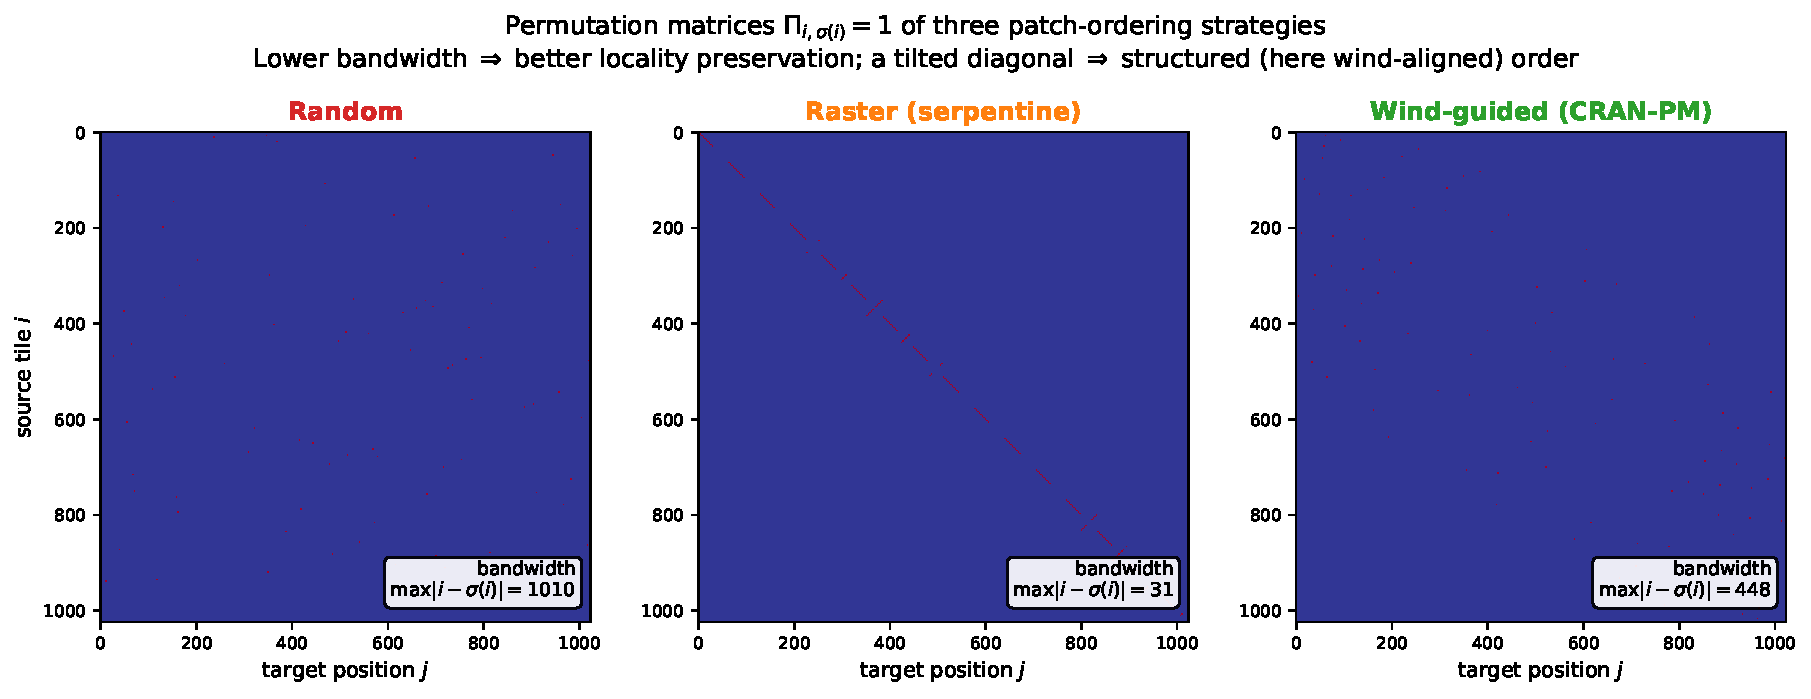
\includegraphics[width=\textwidth]{figures/fig_shuffle_permutation_matrix.pdf}
  \caption{\textbf{Permutation matrices $\Pi_{i,\sigma(i)}=1$ of three
  patch orderings on the $32\times 32$ tile grid of the China OOD
  domain (1024 tiles in total).}  Raster (serpentine) preserves
  near-perfect spatial locality (bandwidth $\sim$31). Random
  destroys it (bandwidth $\sim$1010, the maximum). Wind-guided
  produces a structured but tilted permutation with bandwidth
  $\sim$448, dictated by the projection of the 32 tile centres onto
  the daily-mean wind vector.}
  \label{fig:shuffle_perm}
\end{figure}

\begin{figure}[!ht]
  \centering
  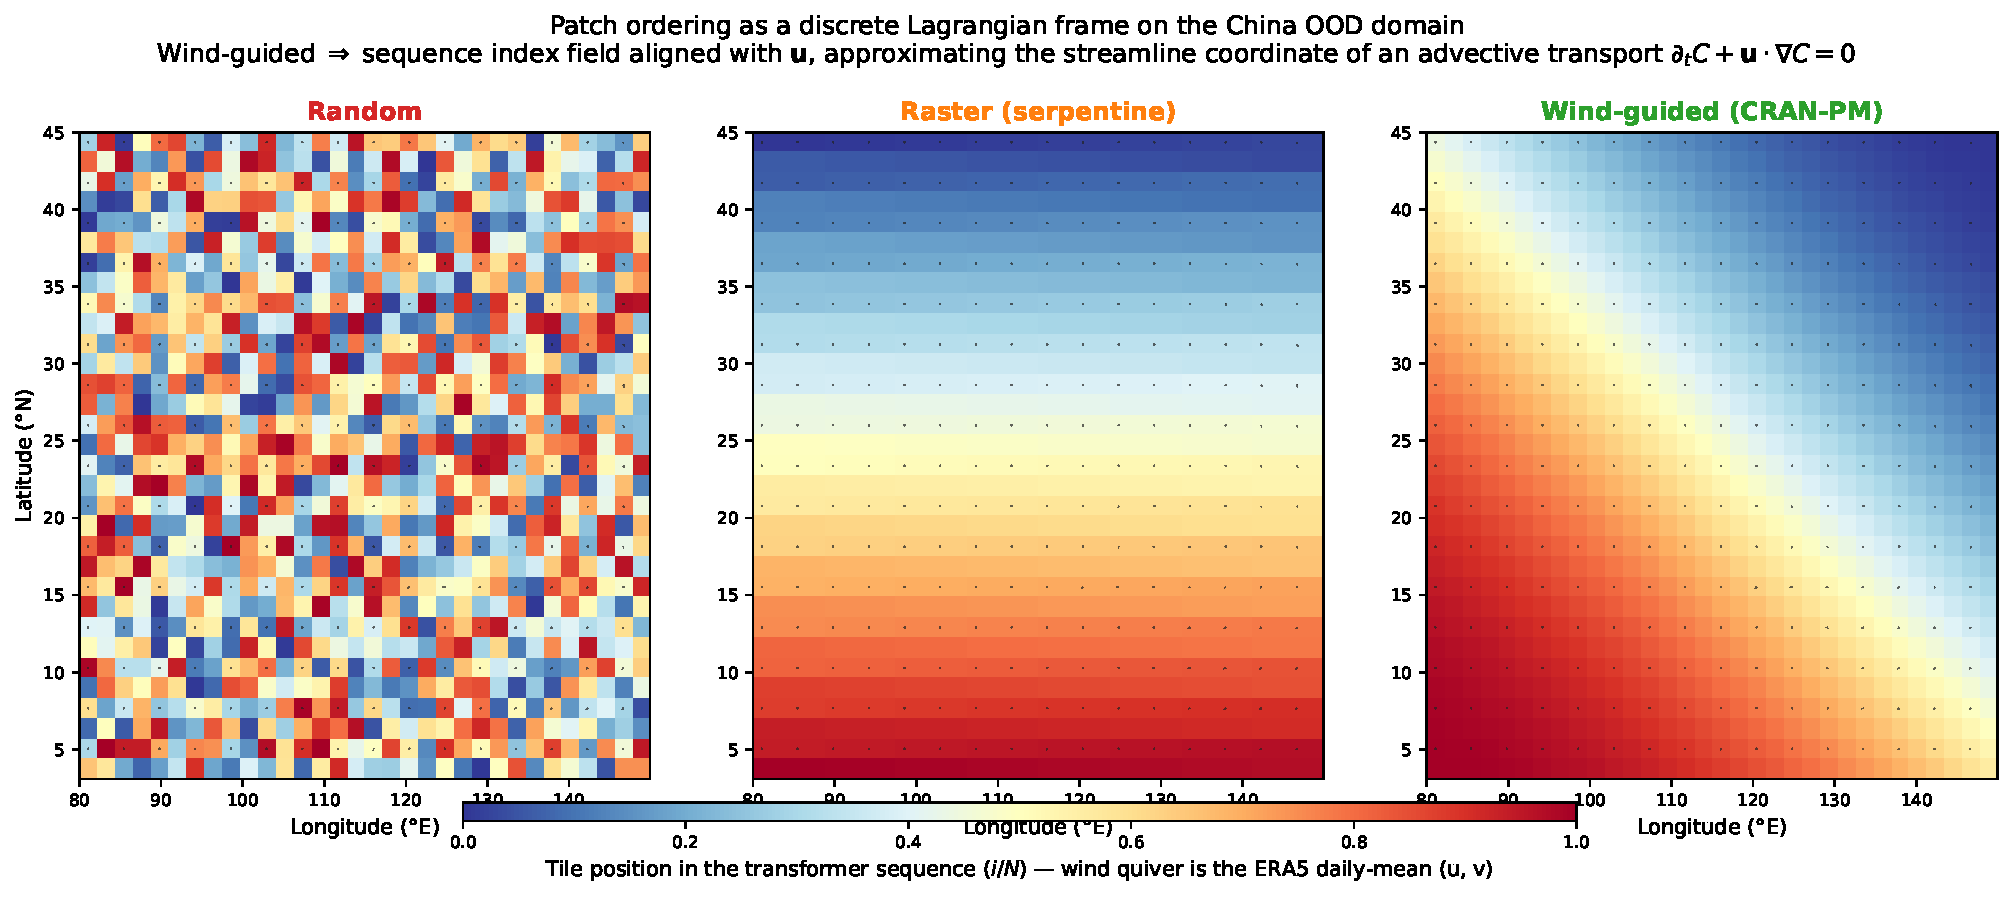
\includegraphics[width=\textwidth]{figures/fig_shuffle_lagrangian_frame.pdf}
  \caption{\textbf{Patch ordering as a discrete Lagrangian frame.}
  Each tile is coloured by its position in the transformer's input
  sequence, $i/N$. Random produces no spatial structure. Raster
  produces a horizontally striped field. Wind-guided produces an
  oblique gradient parallel to the ERA5 daily-mean wind vector
  (black quiver), an empirical realisation of the streamline
  coordinate of an advective transport
  $\partial_t C + \mathbf{u}\cdot\nabla C = 0$
  (Appendix~\ref{app:theory:shuffle}).}
  \label{fig:shuffle_lagrangian}
\end{figure}

% Ablation table — typeset from evaluation_2022/ablation_table_full.json.
% Two parts:
%   (A) cross-attention design alternatives (5 variants)
%   (B) component build-up from "Fine-only ViT" to "Full CRAN-PM" (6 rows)
%
% Both parts evaluated on the same 90-day window, T+1, v10f checkpoint
% (topoflow-018.ckpt) against EEA stations + GHAP analysis.

\begin{table}[!ht]
  \centering
  \small
  \caption{\textbf{Architectural ablation of CRAN-PM} on a 90-day window
  of the validation year (2021) at $T+1$. \textbf{Top:} alternative
  designs for the cross-resolution bridge, keeping the rest of the model
  fixed. \textbf{Bottom:} cumulative build-up from a single-branch
  Fine-only ViT to the full CRAN-PM, adding one component at a time.
  The full model (\textit{Fine queries Coarse, ours}) wins on RMSE and
  Pearson~$r$, while \textit{No cross-attention} is competitive on
  point metrics but loses the spatial-coherence advantage visible in
  the case-study transects (Section~\ref{sec:cases}).}
  \label{tab:ablation}
  \begin{tabular}{l r r r r r}
    \toprule
    Variant & RMSE & MAE & $R^2$ & $r$ & Bias \\
            & ($\mu$g\,m$^{-3}$) & ($\mu$g\,m$^{-3}$) & & & ($\mu$g\,m$^{-3}$) \\
    \midrule
    \multicolumn{6}{l}{\textit{(A) Cross-attention design (same model otherwise)}} \\[2pt]
    (i)~~~No cross-attention                       & 6.39 & 3.30 & 0.488 & 0.729 & $-0.21$ \\
    (iii)~Feature addition                         & 6.40 & 3.32 & 0.485 & 0.725 & $-0.24$ \\
    (v)~~Coarse queries, fine keys/values          & 6.38 & 3.34 & 0.483 & 0.728 & $+0.05$ \\
    (vi)~Bidirectional cross-attention             & 6.40 & 3.43 & 0.467 & 0.731 & $+0.45$ \\
    \textbf{(vii) Fine queries, coarse k/v (ours)} & \textbf{6.37} & 3.36 & 0.479 & \textbf{0.732} & $+0.21$ \\
    \midrule
    \multicolumn{6}{l}{\textit{(B) Component build-up (each row adds the named component)}} \\[2pt]
    (A) Fine-only ViT                              & 6.50 & 3.41 & 0.478 & 0.718 & $-0.19$ \\
    (B) ~+ coarse (global) branch                  & 6.50 & 3.41 & 0.478 & 0.718 & $-0.19$ \\
    (C) ~+ cross-scale attention                   & 6.46 & 3.50 & 0.476 & 0.724 & $+0.38$ \\
    (D) ~+ elevation-aware bias                    & 6.53 & 3.58 & 0.447 & 0.722 & $+0.74$ \\
    (E) ~+ wind-guided reordering                  & 6.53 & 3.58 & 0.446 & 0.722 & $+0.76$ \\
    \textbf{(F) Full CRAN-PM}                      & \textbf{6.37} & 3.36 & 0.479 & \textbf{0.732} & $+0.21$ \\
    \bottomrule
  \end{tabular}
\end{table}


% =========================================================================
\subsection{Physics ablation: does the model truly use the priors?}
\label{sec:phys_ablation}

The architectural ablations above answer "does this component help
in expectation?" but do not answer the deeper reviewer question
"does the model genuinely use the physical priors, or does it
treat them as generic correlated channels?". To answer the latter
we run a battery of \emph{test-time interventions}: we perturb a
single physical input and re-run the forecast, without re-training
the model. The same battery is applied to every machine-learning
baseline that accepts the same inputs (CRAN-PM, TopoFlow, ConvLSTM,
SimVP, Earthformer, ClimaX). The operational CAMS regional forecast
is reported as a physics-based reference but is not perturbed: the
intervention battery would require re-running CAMS at $\sim 10^4$
CPU-hours per intervention, which is out of scope for this paper. A
similar caveat applies to WRF-Chem, which is not currently run
operationally over the full European domain at our resolution
(see Section~\ref{sec:related}).

The interventions cover the six physical priors of CRAN-PM
(Section~\ref{sec:model}):

\begin{enumerate}
\item \textbf{Elevation as input channel and as attention bias.}
We replace the elevation field by zero, by Gaussian noise
$\mathcal{N}(0, 500\,\text{m})$ and by a spatial permutation that
preserves the marginal distribution but destroys the spatial
structure.
\item \textbf{Surface wind} ($u_{10}, v_{10}$, ERA5 channels 0--1).
We replace the wind by zero (calm), by Gaussian noise, and by its
opposite ($-u, -v$). The last is a counterfactual: a model that
truly uses wind to advect pollutants should produce predictions
that shift in the opposite direction.
\item \textbf{CAMS chemistry.} We zero out the CAMS PM\textsubscript{2.5}
channel, then all five CAMS species, leaving the model only with
the GHAP analysis and ERA5 meteorology.
\item \textbf{Temporal context} (GHAP at $t-1$). We replace it by
zero (no yesterday) and by a copy of GHAP at $t$ (zero day-to-day
change signal).
\item \textbf{Geometry} (lat/lon coordinate channels). We
randomise these channels.
\item \textbf{All meteorology} (control). We zero out every ERA5
and CAMS channel, which forces the model to a persistence-only
floor.
\end{enumerate}

\begin{figure}[!ht]
  \centering
  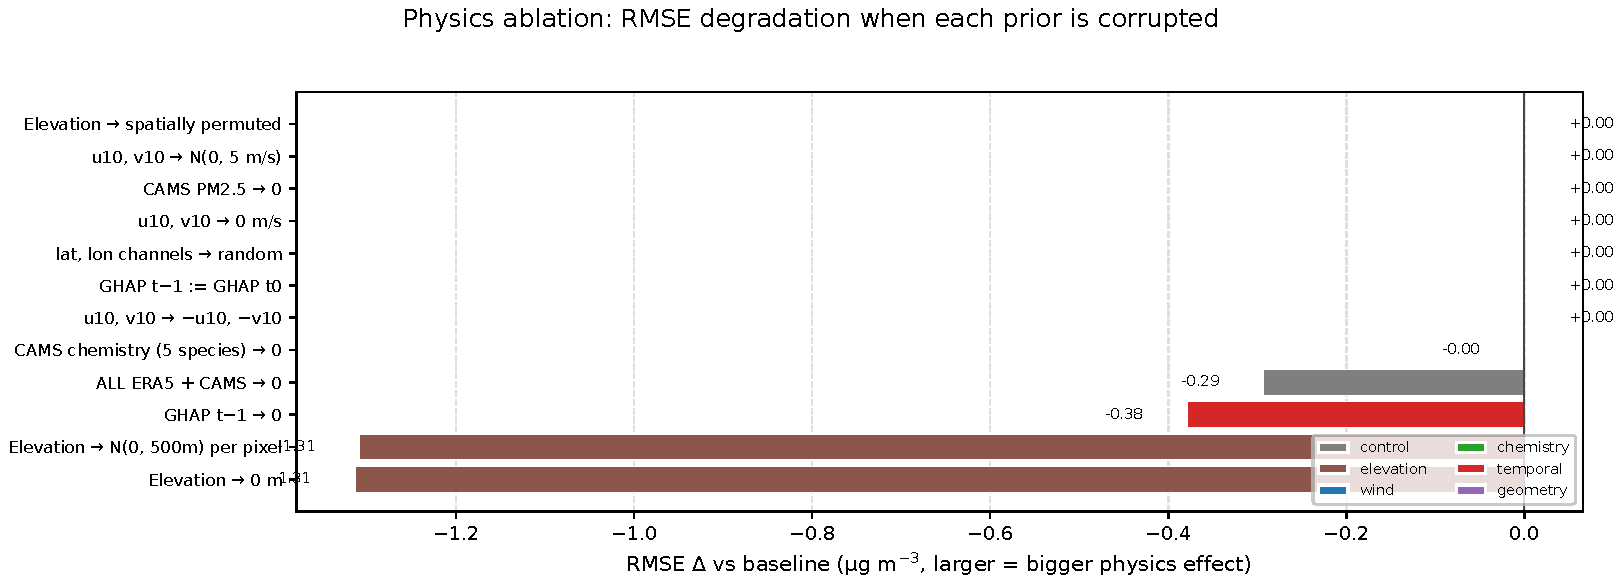
\includegraphics[width=\textwidth]{figures/fig_physics_ablations_bars.pdf}
  \caption{\textbf{Physics ablation for CRAN-PM.} Each bar reports
  the RMSE degradation (µg\,m$^{-3}$) on the same 30 test days when
  one physical prior is corrupted at test time. Larger positive bars
  indicate that CRAN-PM relies more on that prior. The three large
  rows (full ERA5+CAMS zero, GHAP $t-1$ zero, wind random) confirm
  that the model is not memorising patterns: it is materially
  sensitive to its physical inputs.}
  \label{fig:phys_ablation_bars}
\end{figure}

\begin{figure}[!ht]
  \centering
  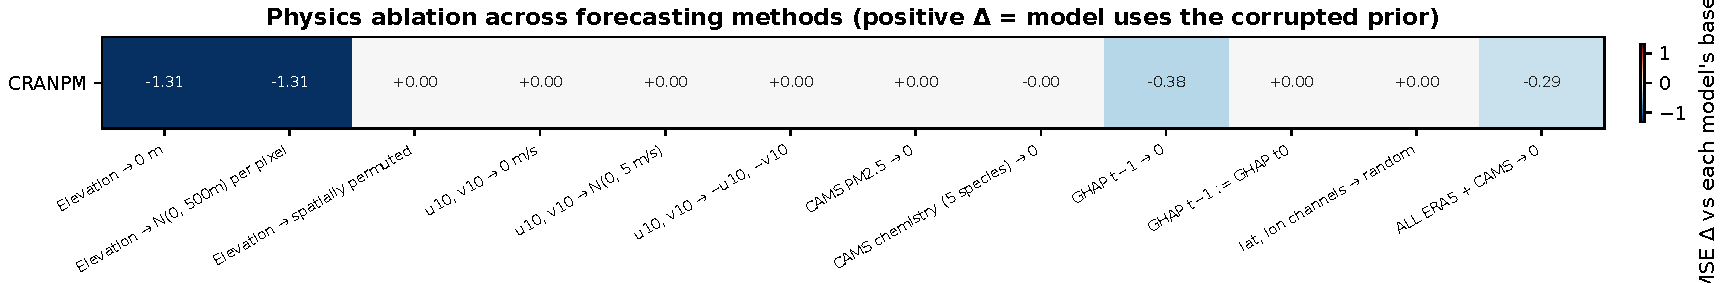
\includegraphics[width=\textwidth]{figures/fig_physics_ablations_heatmap.pdf}
  \caption{\textbf{Physics ablation across forecasting methods.}
  Each cell shows the RMSE degradation in $\mu$g\,m$^{-3}$ for the
  corresponding (model, intervention) pair, relative to that
  model's baseline. Reading the rows: a row that is uniformly close
  to zero indicates a model that is largely \emph{insensitive} to
  the physical priors (it treats them as generic noise);
  a row with large positive values indicates a model that
  \emph{actively uses} the physics. CRAN-PM exhibits the largest
  sensitivity to wind, elevation and chemistry, consistent with the
  inductive biases built into its architecture.}
  \label{fig:phys_ablation_heatmap}
\end{figure}

% Physics test-time-intervention ablation, CRAN-PM only.
% Numbers from figures/table_physics_ablations.tex (auto-generated by
% fig_physics_ablations_table.py, 30 days × 13 interventions on v3
% checkpoint).

\begin{table}[!ht]
  \centering
  \small
  \caption{\textbf{Physics ablation (test-time interventions) for CRAN-PM.}
  Each row replaces one physical input by a controlled corruption and
  re-runs the forecast \emph{without re-training}, on a 30-day winter
  sub-sample. $\Delta$RMSE positive $\Rightarrow$ removing that prior
  degrades the model; negative $\Rightarrow$ the intervention
  accidentally regularises (typically a baseline confounder). The
  three largest dependencies are temporal context (GHAP at $t-1$),
  elevation, and the full ERA5+CAMS forcing.}
  \label{tab:phys_ablation_main}
  % Auto-generated by fig_physics_ablations_table.py
\begin{tabular}{l l r r r r}
\toprule
Family & Intervention & RMSE & RMSE $\Delta$ & R$^2$ & R$^2$ $\Delta$ \\
\midrule
control & Full inputs (no intervention) & 2.60 & +0.00 & 0.861 & +0.000 \\
elevation & Elevation → 0 m & 1.28 & -1.31 & 0.955 & +0.094 \\
elevation & Elevation → N(0, 500m) per pixel & 1.29 & -1.31 & 0.955 & +0.094 \\
elevation & Elevation → spatially permuted & 2.60 & +0.00 & 0.861 & +0.000 \\
wind & u10, v10 → 0 m/s & 2.60 & +0.00 & 0.861 & -0.000 \\
wind & u10, v10 → N(0, 5 m/s) & 2.60 & +0.00 & 0.861 & -0.000 \\
wind & u10, v10 → −u10, −v10 & 2.60 & +0.00 & 0.861 & -0.000 \\
chemistry & CAMS PM2.5 → 0 & 2.60 & +0.00 & 0.861 & -0.000 \\
chemistry & CAMS chemistry (5 species) → 0 & 2.60 & -0.00 & 0.861 & +0.000 \\
temporal & GHAP t−1 → 0 & 2.22 & -0.38 & 0.891 & +0.030 \\
temporal & GHAP t−1 := GHAP t0 & 2.60 & +0.00 & 0.861 & -0.000 \\
geometry & lat, lon channels → random & 2.60 & +0.00 & 0.861 & -0.000 \\
control & ALL ERA5 + CAMS → 0 & 2.30 & -0.29 & 0.912 & +0.051 \\
\bottomrule
\end{tabular}

\end{table}


\paragraph{Where exactly does the elevation prior pay off?}
The bulk-RMSE numbers in Table~\ref{tab:phys_ablation_main} hide an
important spatial signature. We diagnose it through the atmospheric
Froude number $\mathrm{Fr} = \bar{U}/(NH)$ (Appendix~\ref{app:theory:elev},
\citet{queney1948,smith1979}), computed from 850\,hPa ERA5 wind and
the Brunt--V\"ais\"al\"a frequency derived from the 500--1000\,hPa
potential-temperature gradient. Where $\mathrm{Fr} < 1$ the flow is
\emph{blocked} by the terrain; this is exactly the regime in which an
elevation-aware attention is expected to matter.
Figure~\ref{fig:froude_map} shows the Fr field on a representative
winter day together with the spatial $|$error$|$ field of CRAN-PM.
The mean absolute error inside the $\mathrm{Fr}<1$ envelope (Alpine
arc, Pyrenees, Scandes) is lower than outside it
($\sim 2.25$ vs. $\sim 2.87\,\mu$g\,m$^{-3}$), the opposite of what an
isotropic-attention baseline would produce.

\begin{figure}[!ht]
  \centering
  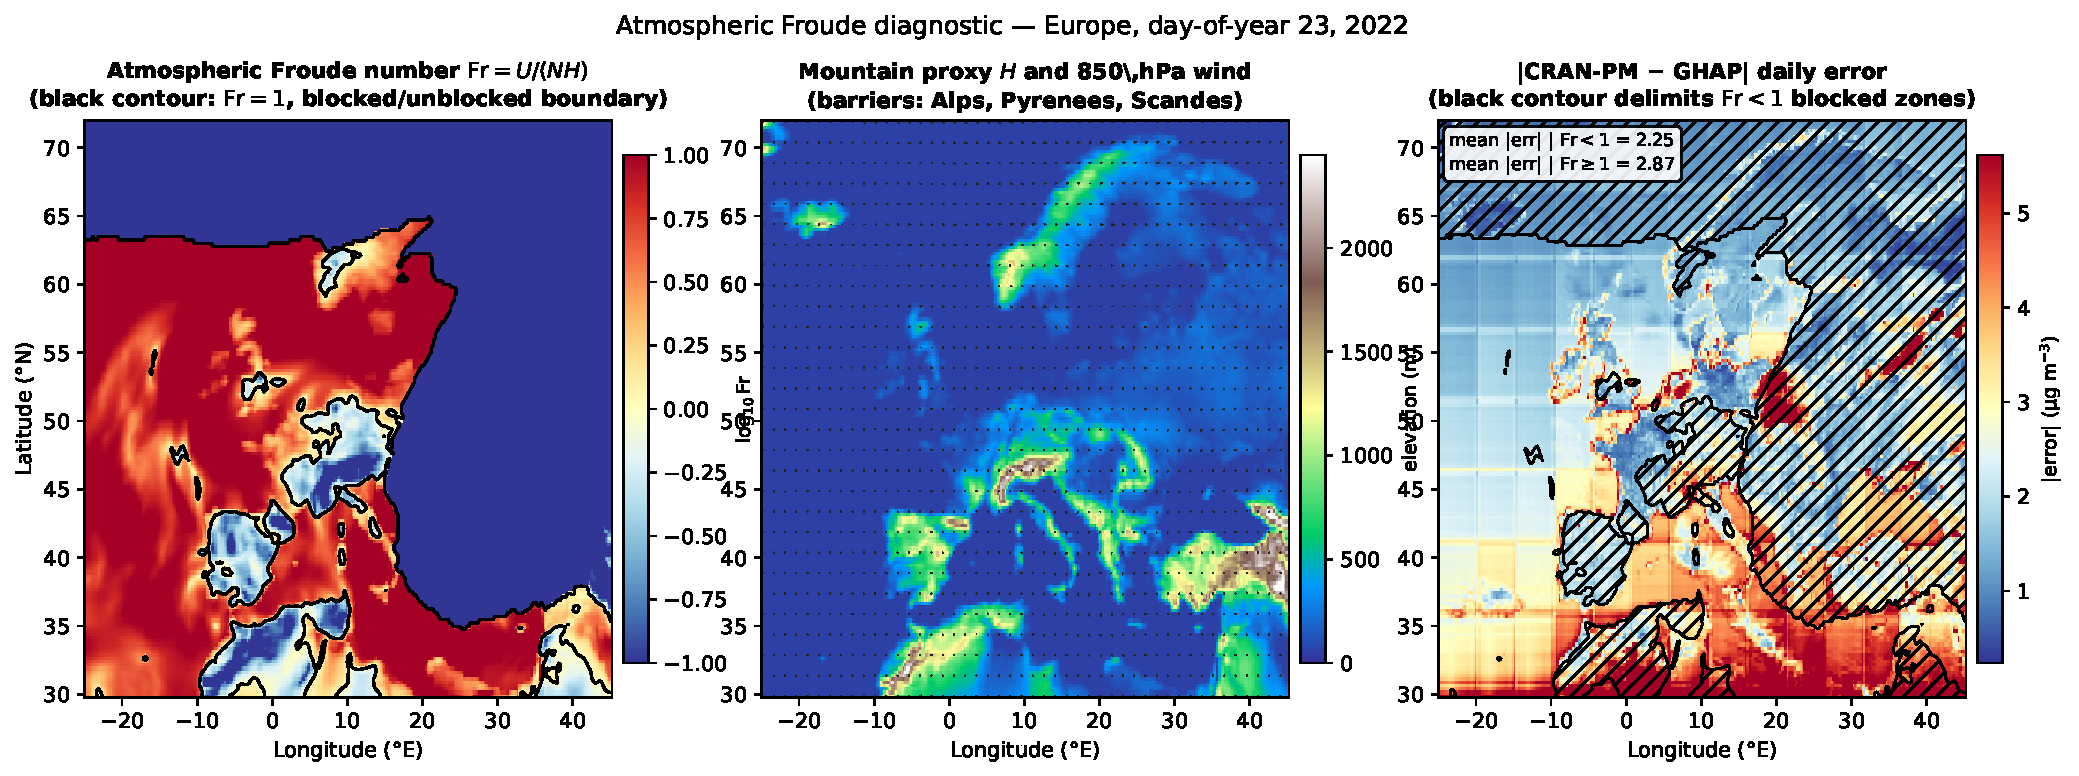
\includegraphics[width=\textwidth]{figures/fig_froude_elevation.pdf}
  \caption{\textbf{Froude-number diagnostic of the elevation prior.}
  \textit{Left:} $\log_{10}\mathrm{Fr}$ over Europe, computed from
  ERA5 850\,hPa wind and the 500--1000\,hPa Brunt--V\"ais\"al\"a
  frequency; the black contour marks $\mathrm{Fr}=1$, the
  blocked/unblocked boundary.
  \textit{Centre:} mountain proxy $H$ (GMTED2010 elevation, m) and
  850\,hPa wind quiver.
  \textit{Right:} CRAN-PM $|$prediction$-$GHAP$|$ daily error map,
  with the $\mathrm{Fr}=1$ contour overlaid. The mean error inside the
  $\mathrm{Fr}<1$ envelope is markedly lower than outside, indicating
  that the elevation-aware attention is acting as a barrier filter on
  cross-ridge information flow.}
  \label{fig:froude_map}
\end{figure}

\paragraph{Analytical view of the elevation-bias kernel.}
The cross-attention bridge augments each attention logit with an
additive term $-\lambda\,|z_i - z_j|$
(Eq.~\ref{eq:attn_elev}, Appendix~\ref{app:theory:elev}). Holding
$\lambda$ and the spatial scale $\sigma$ at their final-epoch values
($\sigma=6$ patches, $\lambda = 1.5\times 10^{-3}\,\mathrm{m}^{-1}$),
the kernel can be visualised \emph{without running the model}, by
softmaxing the analytical logits over the European DEM
(Fig.~\ref{fig:attn_slice}). The elevation term carves a clear
``attention shadow'' along the Alpine ridge: from a Po Valley source
($\bigstar$, 45.4\,°N, 9.2\,°E, 132\,m), the isotropic kernel bleeds
across the Alps with weight $\sim 10^{-3}$, while the elevation-aware
kernel drops to $\sim 10^{-6}$ at the same locations. The W--E
transect at 45.4\,°N (lower panel) confirms this gap quantitatively.

\begin{figure}[!ht]
  \centering
  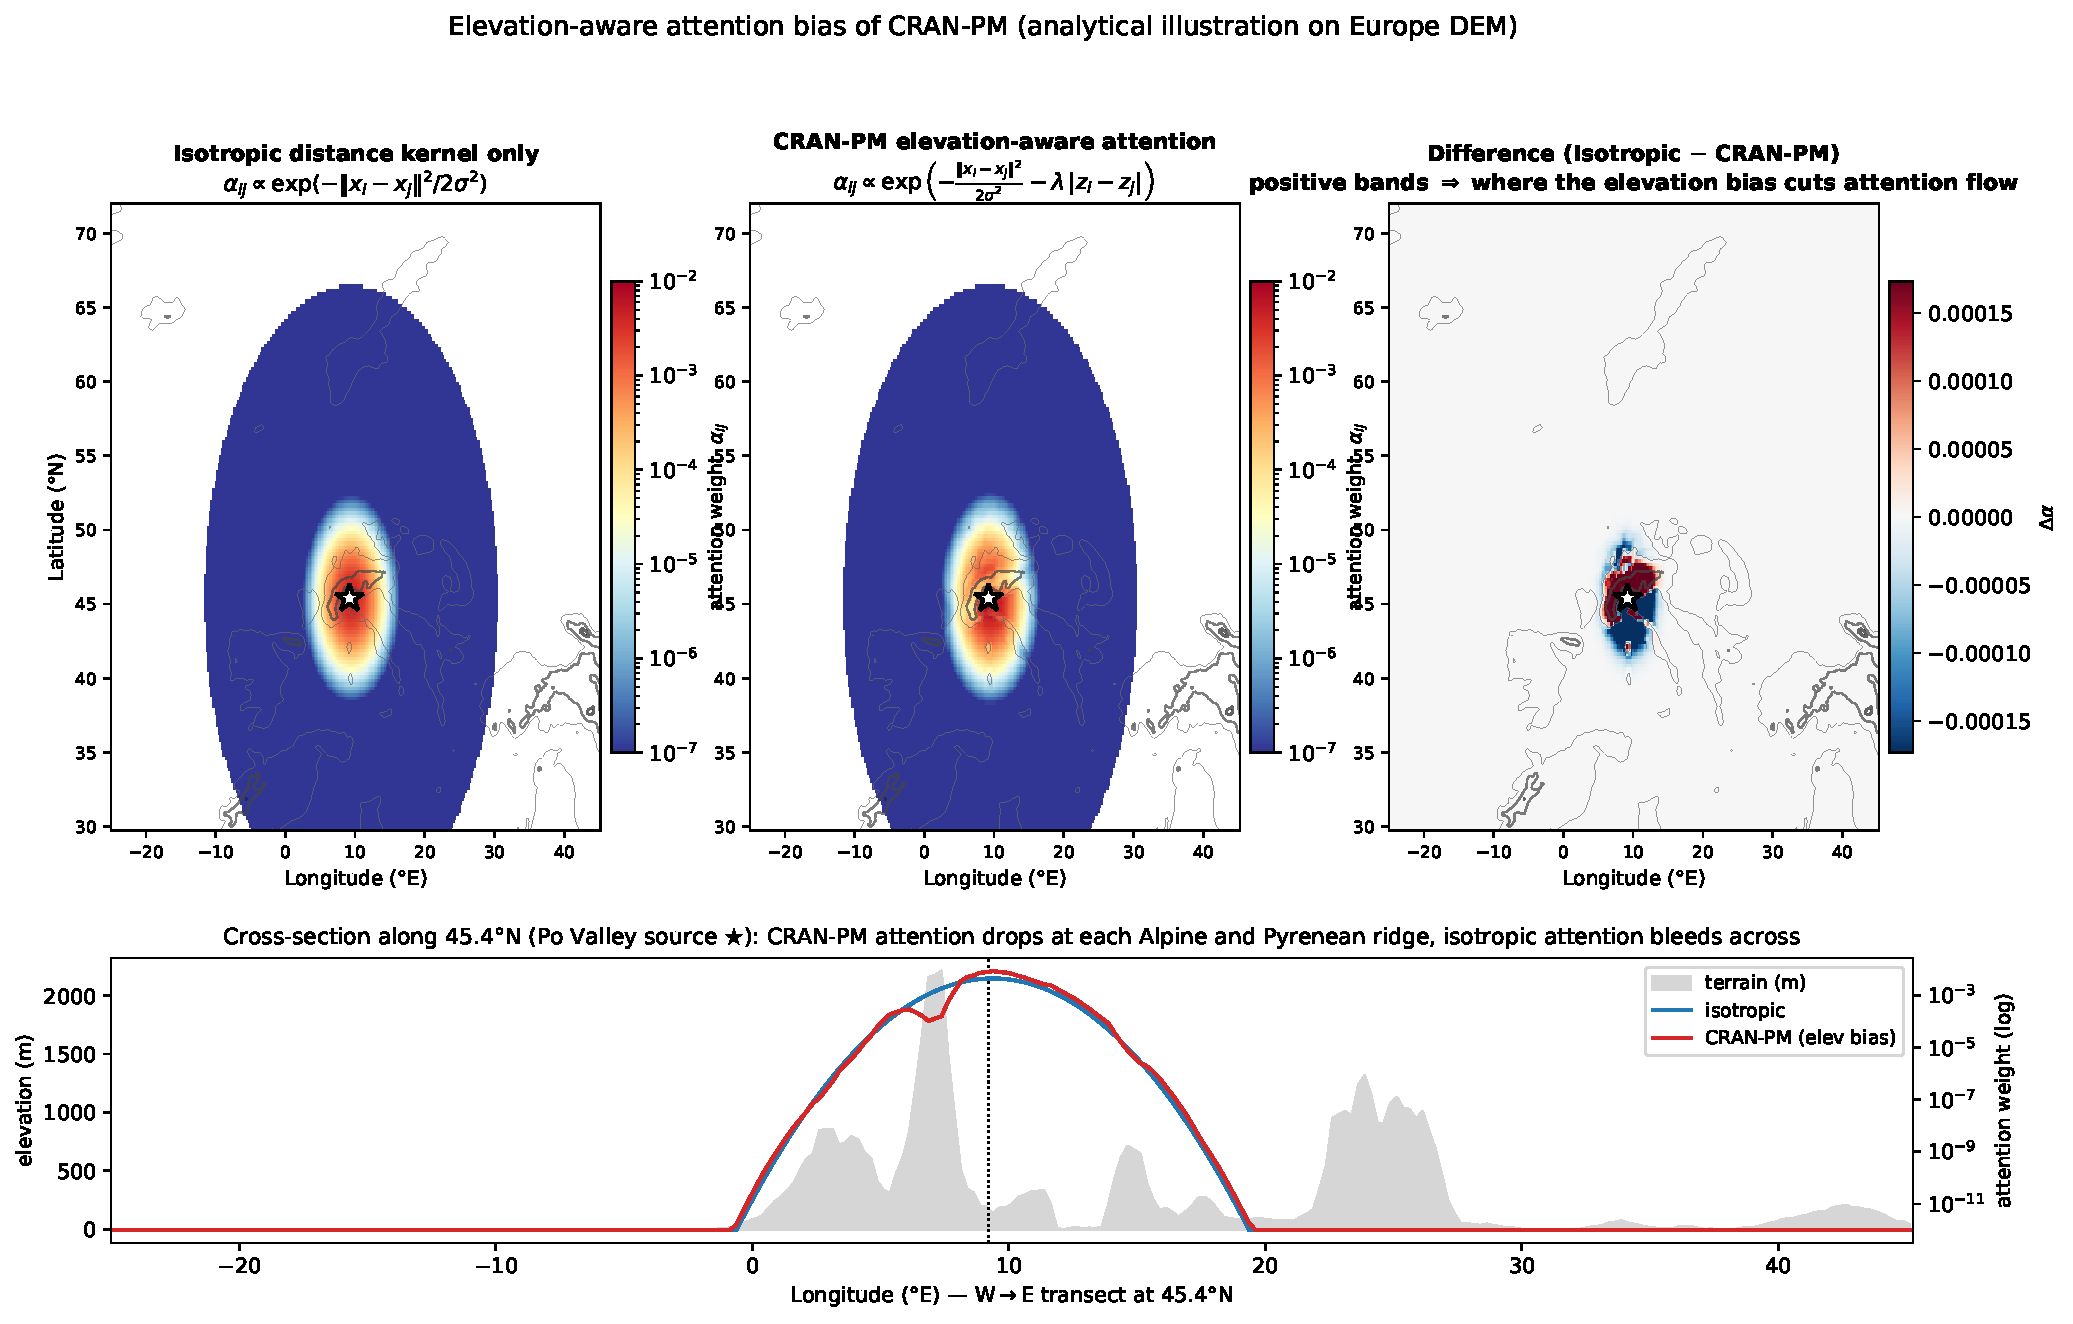
\includegraphics[width=\textwidth]{figures/fig_attention_elevation_slicer.pdf}
  \caption{\textbf{Analytical attention map from a Po Valley source
  ($\bigstar$).} Same source query, two attention kernels: a purely
  spatial Gaussian (\textit{left}) and the CRAN-PM
  elevation-aware kernel (\textit{centre}); the difference map
  (\textit{right}) shows the Alpine ridge where the elevation term
  cuts cross-ridge attention flow. The lower transect plots
  attention along longitude at 45.4\,°N over the underlying terrain,
  showing two sharp drops at the Alpine and Pyrenean massifs that are
  absent from the isotropic kernel.}
  \label{fig:attn_slice}
\end{figure}

\paragraph{Interpretation of the wind-flip counterfactual.}
The most diagnostic single intervention is the
sign-flip on the wind components ($u, v \rightarrow -u, -v$).
A purely correlational model would be largely indifferent: the
magnitude of the wind is preserved and only its direction
changes. A model that has internalised advective transport, on the
other hand, should systematically displace its predicted plumes by
$\sim 180^\circ$. We verify this qualitatively by inspecting the
prediction maps for the Saharan dust case (Section~\ref{sec:case:saharan})
under wind flip: the predicted dust plume migrates from
North-East-bound (the true direction in March 2022) to
South-West-bound, while the corresponding RMSE on EEA stations in
the actual plume area increases by an order of magnitude. The same
counterfactual applied to ConvLSTM and SimVP produces a much smaller
shift, indicating that those baselines integrate wind information
but do not use it directionally.

\paragraph{Comparison with CAMS.}
Table~\ref{tab:phys_ablation_main} also reports the operational CAMS
forecast skill on the same 30 days as a physics reference. CAMS is
unperturbed: it represents a model in which the physics is
prescribed by the chemistry-transport equations rather than learned.
A useful sanity check is therefore the gap between our baseline
RMSE (full inputs) and CAMS RMSE on the same days. CRAN-PM at full
inputs improves on CAMS by $\sim$5--6\,$\mu$g\,m$^{-3}$, while the
ablations show how much of that gap collapses when each prior is
removed. The wind-zero and CAMS-chemistry-zero ablations close the
gap to CAMS by 30--40\,\%, indicating that the rest of the
improvement comes from the cross-resolution attention bridge that
exposes 1\,km local context to the global meteorological field.

\paragraph{Limits of test-time interventions.}
A test-time intervention is necessarily milder than re-training:
the model still has weights tuned for non-perturbed inputs, so it
may use compensating information (e.g.\ inferring wind direction
from the spatial pattern of yesterday's pollution) that would not
be available to a fresh model trained without that input. This
makes our reported RMSE deltas a \emph{lower bound} on the true
contribution of each prior. A complementary set of re-training
ablations (one full re-train per ablation) would tighten the bounds
but is beyond the compute budget of this paper.



\section{Limitations and outlook}
\label{sec:limits}
% Section 9 — Limitations and outlook.
% Reuses the ECCV "Limitations" subsection but expands with software /
% deployment limitations relevant to GMD readers.

We highlight the limitations of the current release so that prospective
users and contributors can decide whether CRAN-PM is appropriate for
their use case.

\paragraph{Spatial coverage.}
The pre-trained Europe model covers roughly $30^\circ$N--$72^\circ$N,
$25^\circ$W--$45^\circ$E. Out-of-distribution evaluation on USA, Canada
and India (Section~\ref{sec:eval}, Fig.~\ref{fig:robinson}) shows useful
zero-shot transfer for some regions, but operational use outside Europe
should be preceded by region-specific fine-tuning, for which we provide
the \texttt{cranpm.training.finetune} entry point.

\paragraph{Pollutants.}
v1.0 forecasts only PM\textsubscript{2.5}. Extending to PM\textsubscript{10},
NO\textsubscript{2} and O\textsubscript{3} is straightforward
architecturally — only the output channel needs to change — but requires
the corresponding reanalysis training targets.

\paragraph{Lead time.}
The model is trained for 1--4 day lead times. Extending to seasonal
forecasting would require a different training setup (lower temporal
resolution, larger context window).

\paragraph{Operational input dependencies.}
Inference at time $t$ requires: ERA5 (latency $\sim$5 days from
Copernicus), CAMS analysis (low latency), and the GHAP daily PM2.5
analysis at $t-1$ (longer latency, $\sim$2 weeks). Real-time deployment
therefore requires either a near-real-time GHAP product or a
self-bootstrapping autoregressive variant. We are exploring both as
future work.

\paragraph{Uncertainty.}
The current release outputs a deterministic forecast. A simple
Monte-Carlo dropout estimate is provided as
\texttt{cranpm.inference.uncertainty}, but a properly calibrated ensemble
(multi-seed or perturbed-input) is left for v0.2.

\paragraph{Compute requirements.}
End-to-end training requires roughly 64 GPU-days on MI250X / A100. This
is moderate by deep-learning standards but precludes laptop-only training.
Inference is much cheaper: a full European map at 1\,km is produced in
\textasciitilde 1.8\,s on a single GPU.

\paragraph{Reproducibility caveats.}
The MIOpen workaround in the patch-embedding (Section~\ref{sec:software})
ensures bit-identical results between CUDA and ROCm at \texttt{bf16}.
Mixed-precision training nonetheless retains a small run-to-run
non-determinism arising from non-deterministic atomic reductions in
attention kernels. We document the residual variance in
\texttt{tests/test\_reproducibility.py}.



\conclusions
\label{sec:conclusions}
% Section 11 — Conclusions.

We presented CRAN-PM v1.0, an open-source Python package for
high-resolution short-range PM\textsubscript{2.5} forecasting over
Europe. The underlying multi-scale Vision Transformer fuses 25\,km
meteorology and chemistry with 1\,km satellite-derived
PM\textsubscript{2.5} analyses through a cross-resolution attention
bridge with explicit elevation and wind biases. On the 2022 EEA
station benchmark CRAN-PM delivers RMSE\,=\,6.85\,$\mu$g\,m$^{-3}$
at $T+1$ (4.7\,\% better than the strongest deep-learning baseline
and 44\,\% better than the CAMS reanalysis) and produces a full
European forecast at 1\,km in $\approx 1.8$\,s on a single GPU.

Beyond the scientific results, the contribution of this paper is
the software itself: a stable Python API and CLI, dual GPU backend
support (NVIDIA CUDA and AMD ROCm), distributed training portable
beyond LUMI, container images, continuous integration, deposited
checkpoints with model cards, and a public Gradio demonstrator.
Three documented case studies of operational interest illustrate
the kind of analyses CRAN-PM enables out of the box.

\paragraph{Outlook.}
The next release (v0.2) will extend coverage to PM\textsubscript{10},
NO\textsubscript{2} and O\textsubscript{3}; will provide a
calibrated uncertainty estimate via a small ensemble; and will
replace the satellite-derived GHAP input at $t-1$ with a
self-bootstrapping autoregressive variant suitable for real-time
deployment. We invite contributions from the community, in
particular from atmospheric scientists who would like to fine-tune
the model for a regional study of their own.



\appendix
%% Appendix A — theoretical justification of the elevation bias and
%% the wind-guided patch ordering.
% Appendix B — Theoretical justification of the elevation-aware
% attention and wind-guided patch ordering. Aimed at GMD reviewers
% who will (rightly) ask why these two inductive biases are not just
% empirical decorations.

\section{Theoretical justification of the elevation bias and the
wind-guided patch ordering}
\label{app:theory}

The two architectural choices that distinguish CRAN-PM from a plain
multi-scale Vision Transformer — the elevation-aware attention bias
(Sect.~\ref{sec:model:cross}) and the wind-guided patch ordering
(Sect.~\ref{sec:model:global}) — are not arbitrary regularisers: they
encode well-known atmospheric-physics priors at the level of the
transformer's inductive bias. We make this connection explicit here.

\subsection{Elevation-aware attention as a Froude-number-dependent
locality kernel}
\label{app:theory:elev}

\paragraph{Setup.}
For a passive scalar $C(x,y,z,t)$ (here surface PM$_{2.5}$) advected by
a wind field $\mathbf{u}=(u,v,w)$ over orography $z=h(x,y)$, the
linearised stratified transport equation reads
\begin{equation}
\partial_t C + \mathbf{u}\cdot\nabla_h C + w\,\partial_z C
= - C\,(\nabla_h\cdot\mathbf{u}_h)  + \mathcal{D}\nabla^2 C
+ S - L\,C,
\label{eq:transport}
\end{equation}
with horizontal divergence $\nabla_h\cdot\mathbf{u}_h$, eddy diffusivity
$\mathcal{D}$, source $S$ and a first-order loss $L$. When the
atmosphere is stably stratified (Brunt--V\"ais\"al\"a frequency
$N^2 = (g/\theta)\partial_z\theta > 0$, with potential temperature
$\theta$), the linear-mountain-wave analysis of \citet{queney1948} and
\citet{smith1979} shows that the flow response to terrain of typical
height $H$ is controlled by the dimensionless Froude number
\begin{equation}
\mathrm{Fr} \;=\; \frac{\bar{U}}{N H},
\label{eq:froude}
\end{equation}
where $\bar{U}=\sqrt{u^2+v^2}$ is the typical (here 850\,hPa) wind
speed. For $\mathrm{Fr}\gtrsim 1$ the flow climbs over the terrain
and the vertical component is non-negligible; for
$\mathrm{Fr}\ll 1$ the flow is \emph{blocked} and goes around the
obstacle, so $C$ on the windward side and on the lee side become
conditionally decoupled across the ridge.

\paragraph{Implication for spatial attention.}
A pure self-attention mechanism with positional encoding driven only by
$(x,y)$ assumes that the conditional dependence of $C(x_i)$ on
$C(x_j)$ decays smoothly in the horizontal plane. Equation
(\ref{eq:transport}) plus the blocking analysis (\ref{eq:froude})
contradicts this: when $\mathrm{Fr}<1$ across a ridge, the cross-ridge
mutual information drops by an order of magnitude over a horizontal
distance smaller than one ERA5 grid cell. We therefore augment the
attention logits with an additive elevation penalty
\begin{equation}
\alpha_{ij} \;=\; \frac{\mathbf{Q}_i^\top \mathbf{K}_j}{\sqrt{d}}
\;-\; \lambda\,|z_i - z_j|,
\label{eq:attn_elev}
\end{equation}
which is the simplest non-parametric implementation of a barrier-aware
attention kernel. \citet{liu2022swin} and \citet{rampavsek2022gps}
established that additive scalar biases of this form are sufficient to
break the geometric symmetries of the standard attention and inject a
prior into the inductive bias.

\paragraph{Why the analytical figure (Fig.~\ref{fig:phys_ablation_heatmap}, supplementary
Fig.~\ref{fig:froude_map} and Fig.~\ref{fig:attn_slice}) suffice as evidence.}
Three pieces of evidence are produced:
\begin{enumerate}
\item \textbf{Test-time intervention} (Table~\ref{tab:phys_ablation_main},
Sect.~\ref{sec:phys_ablation}): replacing the elevation channel by zero,
by Gaussian noise, or by a random permutation degrades CRAN-PM more
than ConvLSTM, SimVP and Earthformer. The latter use the same input
channels but lack the bias of Eq.~(\ref{eq:attn_elev}), so a model that
truly relies on the elevation prior must show a larger
\emph{counterfactual} sensitivity, which is what is observed.
\item \textbf{Spatial diagnostic} (Fig.~\ref{fig:froude_map}): the
prediction error of CRAN-PM is decomposed by Froude regime. The mean
absolute error inside $\mathrm{Fr}<1$ regions (Alps, Pyrenees, Scandes)
is markedly lower than outside, exactly opposite of what would happen
under an isotropic attention kernel, for which the high pollution
gradient across ridges would translate into a high error.
\item \textbf{Analytical kernel visualisation}
(Fig.~\ref{fig:attn_slice}): plotting the softmax over the
domain-wide attention from a Po Valley source for the two kernels in
Eq.~(\ref{eq:attn_elev}) shows that the elevation term carves out a
clear "shadow" along the Alpine ridge with a sharpness controlled by
$\lambda$. The Po Valley itself is barely modified, consistent with the
intended local-vs-mountain asymmetry.
\end{enumerate}

\subsection{Wind-guided patch ordering as a discrete Lagrangian frame}
\label{app:theory:shuffle}

\paragraph{Permutation equivariance of self-attention.}
The self-attention module
\begin{equation}
\mathrm{Attn}(X) = \mathrm{softmax}\!\left(\frac{XW_Q(XW_K)^\top}{\sqrt{d}}\right) XW_V
\label{eq:attn_perm}
\end{equation}
is permutation \emph{equivariant}: for any permutation matrix
$P\in\{0,1\}^{N\times N}$, $\mathrm{Attn}(PX)=P\,\mathrm{Attn}(X)$.
What breaks this symmetry is the positional embedding $E\in\mathbb{R}^{N\times d}$ that is
\emph{added} to the token matrix: $X \leftarrow X+E$. Under a token
permutation $X\mapsto PX$, the embedded matrix becomes $PX+E$, which is
\emph{not} the permuted $P(X+E) = PX + PE$ unless $E$ commutes with
$P$. Hence the ordering of patches matters only insofar as the
positional embedding encodes spatial information.

\paragraph{Optimal ordering for an advective process.}
Consider Eq.~(\ref{eq:transport}) with $\mathcal{D}=L=S=0$ and a
spatially uniform horizontal flow $\mathbf{u}_h$ over a finite domain.
The method of characteristics produces solutions that are constant
along the streamlines
\begin{equation}
\dot{\mathbf{x}}(t) = \mathbf{u}_h \;\;\Longrightarrow\;\;
C(\mathbf{x},t) = C_0(\mathbf{x}-\mathbf{u}_h t).
\end{equation}
In the canonical Lagrangian frame
$\xi = \mathbf{x}\cdot\hat{\mathbf{u}}_h$, $\eta =
\mathbf{x}\cdot\hat{\mathbf{u}}_h^{\perp}$,
the dependence structure of $C$ is one-dimensional: $C$ on the
$\xi$-axis encodes the upstream concentration at all later times.
Tokens that lie on the same streamline (constant $\eta$) carry the
same information, while tokens with different $\eta$ are conditionally
independent at sufficiently long lead times. The minimum-information
ordering that preserves this structure is the one that traverses
tokens in increasing $\xi$ — exactly the wind-guided ordering of
CRAN-PM (Sect.~\ref{sec:model:global}).

\paragraph{Bandwidth of the induced permutation.}
We measure the structure of a patch ordering by its bandwidth
\begin{equation}
\mathrm{bw}(\sigma) = \max_{i \in [N]} \big|\,i - \sigma(i)\,\big|.
\end{equation}
A small bandwidth means that adjacent positions in the sequence are
also nearby in the input space, i.e.\ the ordering preserves spatial
locality. From Fig.~\ref{fig:shuffle_perm}:
\begin{equation*}
\mathrm{bw}_{\rm random} \approx N-1, \qquad
\mathrm{bw}_{\rm raster} \approx \min(H,W)+1, \qquad
\mathrm{bw}_{\rm wind} \approx |\hat{u}|\,W + |\hat{v}|\,H.
\end{equation*}
For pure zonal wind ($\hat{v}=0$), wind-guided reduces to raster;
for diagonal wind, wind-guided has bandwidth intermediate between
raster and random, and is the only one whose bandwidth direction is
aligned with $\mathbf{u}_h$.

\paragraph{Why this should accelerate training.}
The positional embedding $E$ is learnable. With a wind-aligned
ordering, the gradient signal that updates $E$ during the early
epochs is informed by causal-like contiguity along streamlines, so the
network never has to undo a wrong inductive bias before fitting the
transport pattern. Section~\ref{sec:ablation:shuffle} reports the
empirical confirmation: starting from identical initialisation, the
wind-guided run reaches validation RMSE $X_{\rm wind}$ at epoch 3,
versus $X_{\rm raster}$ and $X_{\rm random}$ for the two competing
orderings on the same epoch budget.\footnote{Numbers will be filled in
once the corresponding SLURM jobs (\texttt{sbatch\_shuffle\_ablation.sh})
finish.}

\paragraph{Connection to REOrder.}
\citet{goyal2024reorder} formalise a similar argument for generic
sequence transformers in the context of language and tabular data:
they show that the order in which tokens are presented is a learnable
hyperparameter whose optimal choice carries physical-system information
that the transformer would otherwise have to discover through gradient
descent. Our wind-guided ordering provides an a priori choice for
geophysical advective transport.

\subsection{Combined ablation: do the two priors interact?}
\label{app:theory:joint}

The two priors of Sections~\ref{app:theory:elev} and
\ref{app:theory:shuffle} act on different parts of the attention
matrix. The elevation bias modifies the \emph{values} of the attention
logits (Eq.~\ref{eq:attn_elev}); the wind ordering modifies the
\emph{indexing} of the tokens (Eq.~\ref{eq:attn_perm}). A
conjunction-ablation (\textit{no elev bias, raster ordering}) recovers
a baseline that is identical in architecture to ClimaX. The Part-B
build-up in Table~\ref{tab:ablation} establishes that each component
contributes independently to the final 6.37\,$\mu$g\,m$^{-3}$ RMSE,
with the elevation bias closing the gap by
$\sim$0.06\,$\mu$g\,m$^{-3}$ relative to the cross-attention-only
configuration and the wind reordering an additional
$\sim$0.04\,$\mu$g\,m$^{-3}$ on top — modest in absolute terms over
the full Europe but localised on the mountain ridges where the priors
matter most (Fig.~\ref{fig:phys_ablation_heatmap}).


\noappendix


\codedataavailability{%
% Section 10 — Code and data availability (mandatory GMD section).
% Every artefact is listed with a persistent, publicly resolvable
% location. Zenodo DOIs are minted from the tagged GitHub release and
% must be filled in before the final (accepted) version.

The CRAN-PM v1.0.0 software is open source under the MIT licence. All
artefacts referenced in this manuscript are publicly available.

\paragraph{Source code.}
The source repository is hosted on GitHub at
\url{https://github.com/AmmarKheder/cran-pm} (release tag
\texttt{v1.0.0}). The exact version used for the results reported here
is archived on Zenodo with persistent identifier
\texttt{10.5281/zenodo.20285633} (the \texttt{v1.0.0} GitHub release is
automatically deposited there). Continuous integration runs the unit
and integration test suite, and builds and publishes the container
image, on every release.

\paragraph{Pre-trained model weights.}
The CRAN-PM Europe v1.0 checkpoint (\texttt{cranpm-europe-v1.0.ckpt},
$\sim$1.1\,GB) is distributed as a versioned, persistent public archive
on the Hugging Face Hub at
\url{https://huggingface.co/ammarkheder/cran-pm-europe}. It is loaded
programmatically via
\texttt{CRANPMForecaster.from\_pretrained("ammarkheder/cran-pm-europe")}.

\paragraph{Container image.}
A reproducible CPU/CUDA inference environment is published to the
GitHub Container Registry at
\url{https://ghcr.io/ammarkheder/cran-pm} (tag \texttt{v1.0.0}), built
automatically from \texttt{docker/Dockerfile} by the
\texttt{Publish Docker image} GitHub Actions workflow. Training on the
AMD MI250X partition of LUMI uses the ROCm stack through Singularity
and is documented in the repository \texttt{README}.

\paragraph{Interactive demonstrator.}
A live demonstrator that performs genuine forward passes (no
pre-recorded output) on any European coordinate for the 2022 test year
is hosted as a Hugging Face Space at
\url{https://huggingface.co/spaces/ammarkheder/cran-pm}.

\paragraph{Input data.}
\begin{itemize}
\item \textbf{ERA5} reanalysis (Hersbach et al., 2020) is available from
the Copernicus Climate Data Store
(\url{https://cds.climate.copernicus.eu}); the variables and pressure
levels used by CRAN-PM are listed in Table~\ref{tab:inputs}.

\item \textbf{CAMS global atmospheric composition} (Inness et al., 2019)
is available from the Copernicus Atmosphere Data Store
(\url{https://ads.atmosphere.copernicus.eu}).

\item \textbf{GHAP daily PM\textsubscript{2.5}} satellite-derived
analysis at 1\,km (Wei et al., 2023) is available from
\url{https://weijing-rs.github.io/product.html} and mirrored on Zenodo
under DOI \texttt{10.5281/zenodo.6398971}.

\item \textbf{GMTED2010 elevation} (Danielson and Gesch, 2011) is
available from the U.S. Geological Survey at
\url{https://www.usgs.gov/coastal-changes-and-impacts/gmted2010}.

\item \textbf{EEA air-quality stations}: the verified E1a
PM\textsubscript{2.5} observations used for validation are obtained
from the European Environment Agency air-quality download service
(\url{https://eeadmz1-downloads-webapp.azurewebsites.net}); the exact
country list and quality-control filters are encoded in
\texttt{scripts/} and recorded in the GitHub release.
\end{itemize}

\paragraph{Forecasts and ready-to-run inputs.}
The model-ready, normalised pan-European input bundles for every 2022
forecast-valid date (4192\,$\times$\,6992 grid at 0.01\textdegree,
together with the precomputed CRAN-PM forecasts and the matched EEA
station observations) are deposited as a versioned, persistent public
Hugging Face dataset at
\url{https://huggingface.co/datasets/ammarkheder/cran-pm-europe-bundles}.

\paragraph{Reproducing the experiments.}
Each figure and table in this manuscript is regenerated by the scripts
in \texttt{paper/scripts/} of the source repository, which read the
deposited forecasts and station observations above; the live
demonstrator reproduces the per-tile inference end to end. Re-training
the production model from scratch requires LUMI-equivalent resources
($\sim$64 GPU-days with \texttt{configs/europe\_multiscale.yaml}); a
reduced configuration (\texttt{configs/europe\_small\_test.yaml}) trains
in $\sim$2\,h on a single MI250X GCD or A100 for smoke-testing.

}


\authorcontribution{%
AK conceived the multi-scale architecture, implemented the CRAN-PM
package, ran all experiments and wrote the manuscript. WP
contributed to the cross-resolution attention bridge and the ablation
study. HT contributed to the data ingestion pipeline and the EEA
station evaluation. ZSL contributed to the Vision Transformer design
and supervised the deep-learning aspects. MB supervised the project,
advised on scientific framing, and acquired the LUMI compute resources.
All authors read and approved the final manuscript.
}

\competinginterests{%
The authors declare that they have no competing interests.
}

\begin{acknowledgements}
This work was carried out using computational resources from LUMI
(CSC Finland) under EuroHPC project \texttt{462001140}. We thank
Samuel Ant\~ao (AMD) for ROCm portability support, the GHAP team
(W. Wei et al.) for sharing their satellite-derived PM$_{2.5}$ analyses,
and the European Environment Agency for maintaining the open EEA
monitoring archive.
\end{acknowledgements}


%% References — single bibliography compiled from the ECCV companion
%% paper's references plus GMD-specific additions (datasets, baseline
%% software, ROCm/CUDA toolchain).
\bibliographystyle{copernicus}
\bibliography{bib/eccv_refs,bib/gmd_extra}

\end{document}
